\documentclass[oneside,11pt,dvipsnames]{book}

\usepackage[utf8]{inputenc}
\usepackage[T1]{fontenc}
\usepackage[margin=1.5in]{geometry}
\usepackage{soul}
% \usepackage[small,compact]{titlesec} %very powerful
\usepackage[most]{tcolorbox}
% \setsecnumdepth{subsection}
% \setcounter{tocdepth}{3}
\usepackage{enumitem}
\usepackage{epigraph}
\usepackage{cite}
\usepackage{caption}
\captionsetup{font=small}
\usepackage{graphicx}
\usepackage{hyperref}
\usepackage{wrapfig}
\setlength\intextsep{0pt} % remove extra space above and below in-line float
\usepackage{hyperref}
\hypersetup{
  colorlinks,
  citecolor=black,
  filecolor=black,
  linkcolor=blue,
  urlcolor=blue,
}
\usepackage{booktabs}


\usepackage{tikz}
\usetikzlibrary{calc}
\usepackage{xcolor}

\usepackage{anyfontsize}
\usepackage{sectsty}

\usepackage[makeroom]{cancel}

\newtcolorbox{mybox}{
  enhanced,
  boxrule=0pt,frame hidden,
  borderline west={2pt}{0pt}{green!75!black},
  colback=green!10!white,
  sharp corners
}

\newenvironment{commentbox}[1][]{
  \small
  \begin{mybox}
    {\small \textbf{#1}}
  }{
  \end{mybox}
}

\newtcolorbox{mydomesticbox}{
  enhanced,
  boxrule=0pt,frame hidden,
  borderline west={2pt}{0pt}{red!75!black},
  colback=blue!10!white,
  sharp corners
}

\newenvironment{domesticbox}[1][]{
  \small
  \begin{mydomesticbox}
    {\small \textbf{#1}}
  }{
  \end{mydomesticbox}
}

\renewcommand{\figurename}{Fig.}
\renewcommand{\tablename}{Tab.}
\def\Section{\S}
\renewcommand{\figureautorefname}{Fig.}
\renewcommand{\tableautorefname}{Tab.}
\makeatletter
\renewcommand{\chapterautorefname}{\S\@gobble}
\renewcommand{\sectionautorefname}{\S\@gobble}
\renewcommand{\subsectionautorefname}{\S\@gobble}
\renewcommand{\appendixautorefname}{\S\@gobble}
\makeatother

\newcommand{\mycomment}[3][\color{blue}]{{#1{{#2}: {#3}}}}
\newcommand{\tvn}[1]{\mycomment{TVN}{#1}}{}
\newcommand{\didi}[1]{\mycomment{Didier}{#1}}{}
\newcommand{\tl}[1]{\mycomment{ThanhLe}{#1}}{}
\newcommand{\red}[1]{{\color{red}{#1}}}
\newcommand{\xz}[1]{\mycomment{Xiaokuan}{[#1]}}{}


\begin{document}

\pagestyle{empty}
\begin{tikzpicture}[overlay,remember picture]

    % Background color
    \fill[
    black!2]
    (current page.south west) rectangle (current page.north east);
    
    % Rectangles
    \shade[
    left color=Dandelion, 
    right color=Dandelion!40,
    transform canvas ={rotate around ={45:($(current page.north west)+(0,-6)$)}}] 
    ($(current page.north west)+(0,-6)$) rectangle ++(9,1.5);
    
    \shade[
    left color=lightgray,
    right color=lightgray!50,
    rounded corners=0.75cm,
    transform canvas ={rotate around ={45:($(current page.north west)+(.5,-10)$)}}]
    ($(current page.north west)+(0.5,-10)$) rectangle ++(15,1.5);
    
    \shade[
    left color=lightgray,
    rounded corners=0.3cm,
    transform canvas ={rotate around ={45:($(current page.north west)+(.5,-10)$)}}] ($(current page.north west)+(1.5,-9.55)$) rectangle ++(7,.6);
    
    \shade[
    left color=orange!80,
    right color=orange!60,
    rounded corners=0.4cm,
    transform canvas ={rotate around ={45:($(current page.north)+(-1.5,-3)$)}}]
    ($(current page.north)+(-1.5,-3)$) rectangle ++(9,0.8);
    
    \shade[
    left color=red!80,
    right color=red!80,
    rounded corners=0.9cm,
    transform canvas ={rotate around ={45:($(current page.north)+(-3,-8)$)}}] ($(current page.north)+(-3,-8)$) rectangle ++(15,1.8);
    
    \shade[
    left color=orange,
    right color=Dandelion,
    rounded corners=0.9cm,
    transform canvas ={rotate around ={45:($(current page.north west)+(4,-15.5)$)}}]
    ($(current page.north west)+(4,-15.5)$) rectangle ++(30,1.8);
    
    \shade[
    left color=RoyalBlue,
    right color=Emerald,
    rounded corners=0.75cm,
    transform canvas ={rotate around ={45:($(current page.north west)+(13,-10)$)}}]
    ($(current page.north west)+(13,-10)$) rectangle ++(15,1.5);
    
    \shade[
    left color=ForestGreen,
    rounded corners=0.3cm,
    transform canvas ={rotate around ={45:($(current page.north west)+(18,-8)$)}}]
    ($(current page.north west)+(18,-8)$) rectangle ++(15,0.6);
    
    \shade[
    left color=ForestGreen,
    rounded corners=0.4cm,
    transform canvas ={rotate around ={45:($(current page.north west)+(19,-5.65)$)}}]
    ($(current page.north west)+(19,-5.65)$) rectangle ++(15,0.8);
    
    \shade[
    left color=OrangeRed,
    right color=red!80,
    rounded corners=0.6cm,
    transform canvas ={rotate around ={45:($(current page.north west)+(20,-9)$)}}] 
    ($(current page.north west)+(20,-9)$) rectangle ++(14,1.2);
    
    % Year
    \draw[ultra thick,gray]
    ($(current page.center)+(5,2)$) -- ++(0,-3cm) 
    node[
    midway,
    left=0.25cm,
    text width=5cm,
    align=right,
    black!75
    ]
    {
    {\fontsize{25}{30} \selectfont \bf Computer\\[8pt] Science}
    } 
    node[
    midway,
    right=0.25cm,
    text width=6cm,
    align=left,
    ForestGreen]
    {
    {\fontsize{48}{50} \selectfont PhD}
    };
    
    % Title
    \node[align=center] at ($(current page.center)+(0,-5)$) 
    {
    {\fontsize{24}{24} \selectfont {{Demystifying the Computer Science}}} \\[0.15in]
    {\fontsize{24}{24} \selectfont {{PhD Admission in the US}}} \\[0.2in]    
    {\fontsize{18}{18} \selectfont {{A Handbook for International Students}}} \\[0.5in]    

    {\fontsize{16}{19.2} \selectfont \textcolor{ForestGreen}{ \bf ThanhVu (Vu) Nguyen}}\\[0.1in]
    George Mason University, Dept. of Computer Science\\[0.1in]
    \today{} (latest version available on  \href{https://github.com/nguyenthanhvuh/phd-cs-us}{Github})
    };
    \end{tikzpicture}

    
\chapter*{Preface}
Having been involved in PhD admission committees for many years, I've realized that many \textbf{international} students, especially those in smaller countries or less well-known universities, lack a clear understanding of
the Computer Science PhD admission process at US universities. This confusion not only
discourages students from applying but also creates the perception that
getting admitted to a CS PhD program in the US is difficult compared to other countries.

% though \emph{very} top schools could be very selective, e.g., see the \href{https://da-data.blogspot.com/2015/03/reflecting-on-cs-graduate-admissions.html}{admission process} at CMU
So I want to share some details about the admission process and advice for those who are interested in applying for a \textbf{PhD in Computer Science in the US}.
Originally, this document was intended for international students, but I have expanded it to include information that might also be useful for \emph{domestic students}.
Moreover, while this handbook is primarily intended for students interested in CS, it might be relevant to students from various disciplines.
Furthermore, although many examples are specifics for schools that I and other contributors of this document know about, the information should be generalizable to other R1\footnote{An \href{https://en.wikipedia.org/wiki/List_of_research_universities_in_the_United_States}{R1 institution} in the US is a research-intensive university with a high level of research activity across various disciplines. Currently, 146 (out of 4000) US universities are classified as R1.} institutions in the US (and universities in other countries).

In addition, this handbook can help \textbf{US faculty and admission committee} gain a better understanding of international students and their cultural differences.  By recognizing and leveraging these differences, CS programs in the US can attract larger and more competitive application pools from international students.

I wish you the best of luck. Happy school hunting!

\begin{mybox}
The latest version of this document is available at

\begin{center}
  \href{https://nguyenthanhvuh.github.io/phd-cs-us/demystify.pdf}{nguyenthanhvuh.github.io/phd-cs-us/demystify.pdf},
\end{center}

\noindent and its \LaTeX{} source is also on \href{https://github.com/nguyenthanhvuh/phd-cs-us}{Github}. If you have questions or comments, feel free to create new \href{https://github.com/nguyenthanhvuh/phd-cs-us/issues}{GitHub issues} or \href{https://github.com/nguyenthanhvuh/phd-cs-us/discussions}{discussions}.

\end{mybox}

\newpage
\tableofcontents

\chapter{Summary}\label{sec:summary}

This section summarizes the main points of this guideline. This gives you an overview to decide which specific topics you want to explore more thoroughly.


\begin{enumerate}
  \item Should you apply?
        \begin{itemize}
          \item \emph{Yes, definitely}.  CS PhD study in the US is fully funded and admission into good universities is not any harder than in other countries (\autoref{sec:should}).
        \end{itemize}
  \item How is your application evaluated?
        \begin{itemize}
          \item Applications are evaluated by the \emph{PhD Admission} (adcom) committee and each application is typically reviewed by three faculty members (\autoref{sec:evalapps}).
          \item Individually faculty \emph{cannot directly admit} a student---so do not email and ask if you have a chance. However, faculty can \emph{advocate} for a student and therefore increase their admission chance---contact and introduce yourself (\autoref{sec:contact}).
         \end{itemize}
  \item Application Materials
        \begin{itemize}
          \item The committee will look at various factors, but the most important ones are letters of recommendation (LORs) and research ability, e.g., publications, statement of purpose (SOP).
          \item \emph{LORs are very important}, but only if they are personalized and talk about your research ability (\autoref{sec:lor}).
          \item \emph{SOP is very important}. Write it in such a way that makes you \emph{stand out} (\autoref{sec:research-statement} and \autoref{sec:improve-your-chance})
          \item  \emph{Publications can greatly help}. Publications in good venues are concrete evidence that you have successfully engaged in research. But they are not required! (\autoref{sec:research-experiences}).

          \item \emph{Grades might be important}, depends on the reputation of \emph{your school} (\autoref{sec:your-school}). While good grades might not help much, bad ones likely will hurt your case.
          
          \item \emph{Standard tests are not important} (\autoref{sec:standard-tests}). GRE typically \emph{is not} required. For standard English tests (not required for domestic students), just do enough to pass the minimum requirements.

          \item \emph{Contacting a prof. is recommended}, but do it \emph{properly} (\autoref{sec:contact}).

          \item Getting an interview is typically a \emph{good sign}; but no interview does not mean rejection (\autoref{sec:interview}).

        \end{itemize}
  \item What to do after getting admitted?
        \begin{itemize}
                \item  Celebrating! Now it is your turn to evaluate the school!
          \item Attend \emph{Open House} to learn more about the place and \emph{interview} profs---they would be much more willing to talk to you now (\autoref{sec:accepted}).
        \end{itemize}
  \item Funding
        \begin{itemize}
          \item TAs, RAs, and fellowships are two main funding sources (\autoref{sec:funding}).  TAs (teaching assistantships) are provided by the department to help with classes (e.g., grading). RAs (research assistantships) are given by profs. to help with their research.  Fellowships, provided by the university, department, or external sources such as government or industry, give move flexibility but are very competitive.
        \end{itemize}
  \item Choosing School and Professors
        \begin{itemize}
          \item Many schools do not offer PhD studies in CS and many CS professors do not advise or graduate PhD students  (\autoref{sec:schoolsandprofs}).
        \end{itemize}

    \item Miscs and FAQS
        \begin{itemize}
          \item Why you were rejected (\autoref{sec:why-rejected})
          \item Increasing admission chance by being unique and standing out (\autoref{sec:improve-your-chance}).
          \item Being in an underrepresented group can help can help (\autoref{sec:urm}).
          \item You can successfully apply to CS PhD even if you have non-STEM background (\autoref{sec:non-stem}).
          \item You do not need an MS degree (\autoref{sec:msrequirement}) to apply for PhD in CS, and it takes about 5--7 years for PhD in CS (\autoref{sec:time}).
          \item Compared to other countries, CS PhD in the US does not require an MS degree but has longer PhD study time (\autoref{sec:non-us-differences}).
          \item How do you call a professor? (\autoref{sec:address})
          \item Your entire PhD program costs about \$400K in total, but you \emph{do not} pay for it (\autoref{sec:ra-cost})
          \item Ask your prof. if they can buy computer equipments and such for your research (\autoref{sec:buying-equipment}).
          \item Despite some miserable stories on social media, many PhD students have good mentors, supportive lab mates, healthy working environment ... and are happy (\autoref{sec:happy}).
        \end{itemize}


    \item Appendices
    \begin{itemize}
      \item Specific advice for domestic students (\autoref{sec:domestic-students}).
      \item How to find research opportunities (\autoref{sec:research-opportunities}).
      \item Cultural differences between US and other countries (\autoref{sec:cultural}).
    \end{itemize}

\end{enumerate}


\mainmatter
\chapter{Should You Apply to a CS PhD Program in the US?}\label{sec:should}

\epigraph{\vspace{-0.2in} Don't make fun of graduate students. They just made a terrible life choice.}{\textsc{The Simpsons}}

International students, especially those from less well-known universities and smaller countries, often wonder if they should apply to a CS PhD program in the US. Specifically, they are worried about the \emph{difficulty} of getting admitted and the \emph{cost} of studying in the US. This section addresses these concerns.


First, applying to a good US university \emph{should not} be any harder than at schools in other countries. In fact, it might even be more flexible since CS PhD in the US \emph{do not} require having an MS or a topic/proposal/adviser in advance. If you believe you have a chance in other countries, e.g., South Korea, Singapore, Germany, UK, Japan, and Australia, then you will surely have a chance in the US as well. \autoref{sec:non-us-differences} compares CS PhD study in the US to other countries.


Second, PhD students in CS \emph{do not} need to worry about funding, especially at good R1
universities in the US. If you are admitted, you will almost certainly
receive \emph{full funding} (\autoref{sec:funding}) to support your study, including tuition,
health insurance, and stipend (i.e., you get paid for your study). Moreover, depending on the university,
you may even receive additional benefits such as summer pay, laptops, (conference/workshop) traveling.


\begin{commentbox}[Vu:]
  One of the reasons I created this document is that my colleagues at GMU are interested in recruiting Vietnamese students and are surprised when seeing very few applications in Vietnam (see \autoref{sec:ack}). Each year our CS PhD program receives about 400 PhD applications, most of which are international but only 4--5 are from Vietnam. In general the number of CS PhD applications from Vietnam to US universities is very low and more would be welcome.
\end{commentbox}


\section{Who is this document for?}

While the information presented here can be useful for all students interested in applying to a CS PhD program in the US, this guideline is primarily intended for \textbf{international students} from \textbf{smaller countries and less well-known universities} (similarly, for domestic students from universities with no PhD programs or limited research experiences). 
Students from top schools with strong research cultures and experiences might already know most of the information presented here.
My goal is to level the playing field by providing information that is not readily available to less privileged students.  I also hope to encourage more students from these countries to apply to CS PhD programs in the US.


%% Vu: *what's a PhD?*  This [[https://matt.might.net/articles/phd-school-in-pictures/][series of pictures]] from [[https://matt.might.net][Matt Might]] illustrates what a PhD means.
%% \end{commentbox}

\section*{Additional Resources}
\begin{itemize}
  \item \href{https://parentheticallyspeaking.org/articles/us-cs-phd-faq/}{Getting a Computer Science PhD in the USA} by Shriram Krishnamurthi
  \item  \href{https://pg.ucsd.edu/PhD-application-tips.htm}{Blog post on PhD Admission} by Philip Guo
  \item   \href{https://talkingtorobots.com/yonatanbisk.html}{PhD Admission post} by Yonatan Bisk (customized for CMU admission)
\end{itemize}

\chapter{How is Your Application Evaluated?}\label{sec:evalapps}

\epigraph{How is education supposed to make me feel smarter? Besides, every time I learn something new, it pushes some of the old stuff out of my brain. Remember when I took that home wine making course, and I forgot how to drive?}{\textsc{The Simpsons}}

After you submit your PhD application (usually around December), it will first be screened
for general requirements, e.g., did you submit your transcripts and standard scores? did your reference writers submit their letters? Usually, this screening process is done through a central university system, i.e., not by faculty from the CS department. If you pass this screen, your application will be forwarded to the CS department for further evaluation. If you don't,  the system will tell you what is missing and what you need to do. So pay attention to your email and check your application status regularly.

\begin{commentbox}[Hakan:]
  At GMU, for full consideration, students should make sure to submit \textbf{ALL} required documents by the application deadline, and should never assume that some required documents (such as official TOEFL scores or official diplomas/transcripts) will be waived by the admissions office. If something is listed and not marked as ``optional'', it is mandatory and they should plan for submitting all those.
\end{commentbox}

Then, applications are reviewed by a \emph{PhD admission committee} (\textbf{adcom}) that consists of faculty members in CS\footnote{In some cases the committee can involve affiliated faculty from different disciplines.}. These adcom members have a wide-range of expertise and background to ensure diverse perspectives in the evaluation process. The size and the review load of the adcom depend on the department size. At GMU, the PhD adcom typically has 15--20 faculty, and each committee member is assigned to review 25--30 applications. Note that most large schools, including GMU, have separate adcoms for MS programs.

Each application is assigned to about 3 faculty members, who will evaluate your profile and reach a consensus.  While the assigned reviewers are the main ones deciding your application, other faculty in the department will likely have access to your application and can provide inputs and opinions on your profile.

The PhD adcom typically involves assistant professors in the department (see \autoref{sec:faculty-types} for various types of faculty). This provides junior faculty the opportunities to recruit students. Some members are tenured faculty. The chair of the committee will likely be a senior faculty, but they will not review individual applications and instead assign them to committee members. The chair will look at various factors such as research interests or mentioning faculty names to assign the applications to appropriate faculty, e.g., I am often assigned to review applicants interested in software engineering.

At GMU, we usually decide that a full-time PhD candidate is either (i) admitted with funding (\autoref{sec:funding}) or (ii) rejected. In other words, in most cases, we either
admit you with full funding or reject your application. In some rare cases, we admit
without funding because you have funding on your own, e.g.,
supported by your government or having external fellowships. We justify
our decision with a summary of your application, where we list
strengths, e.g., a well-known school, and weaknesses, e.g., weak
LORs.

% \didi{Is there more information on typical strengths and common weaknesses of applications. This is especially useful to sophomore and junior students as they still have time to work on those strengths.}
% tvn: the main thing is research experiences


\paragraph{Why CS depts do not waive the application fee?}  Some universities do waive, e.g., Rice for all PhD applicants and many universities for domestic students (\autoref{sec:domestic-students}), however most do not.  In any case, the application fee is typically a requirement of the university. Individual departments and programs do not have the flexibility to waive the application fee, even if they want to.

In my opinion, requiring applicants to pay the fee helps ensure their seriousness, as it filters out non-serious candidates.  Also, most CS programs already receive many applications, and would be overwhelmed if the application process were free.  


% \begin{commentbox}[Hung]
%   The application fee varies between schools, and is about \$70--\$100. I found this number pretty ridiculous. In most cases, there is no proper justification for that amount. Yes, the application fee could act as a filter, but a nominal amount would do the job. While a blanket waiver might not be feasible, universities should extend the eligibility of fee waiver applications to more countries.
% \end{commentbox}


\chapter{Your Application}\label{sec:application}

\epigraph{Son, if you really want something in this life, you have to work for it. Now quiet! They’re about to announce the lottery numbers.}{\textsc{The Simpsons}}


The focus of the admissions committee is to \textbf{evaluate your background and interest in research} to see if you can handle a PhD in CS, which is a \emph{research} degree!. We also aim to determine if you would \textbf{fit into the program}. To evaluate your profile, we consider
the following key indicators.


\section{Letters of Recommendation (LOR)}\label{sec:lor}

\begin{center}
  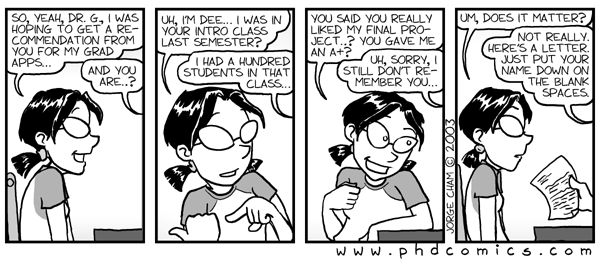
\includegraphics[width=0.6\linewidth]{files/c6.png}
\end{center}


Most PhD programs will require at least \textbf{two LORs}. A good LoR letter should have detail, enthusiasm, and specific examples of the applicant's achievements, all of which paint a compelling picture of the candidate to the adcom.

Having a strong letter from an internationally recognized researcher will \emph{greatly strengthen} your application. A strong letter from a well-known researcher can outweigh the lack of publications (or low GPA or unknown school).
However, obtaining letters from famous people
can be challenging for international students, who might not have many interactions with such experts. So it is fine to have a letter from people (e.g., profs, researchers, postdocs who mentored you) who know you well enough to talk about \emph{your research experience and capabilities}. 

Many students get letters from supervisors from companies where they did internships or are working.  It is OK as long as it is a research-based personalized letter. Again, the emphasis here is \emph{research}, i.e., the letters should describe your research experiences and potential. Letters focusing on your course work or non-research projects at a company won't carry much weight.

\begin{commentbox}[Vu:]
  If your grading system is not US standard or you are from a good school unknown outside your country, you can ask your reference writers to explain that in their letters.  For example, ``Bach Khoa'' are the top universities in Vietnam for STEM studies but few people outside Vietnam know about them.  So if you are from there, you should ask your reference writers to mention that.
\end{commentbox}

\paragraph{How to help your LOR writer} Your LoR writer can ask you to provide additional information to help them write your letter.  For example, they might ask about GPA, research and work experiences, papers (if any), or anything you want them to mention. You can also provide them with a draft of your SOP so that they can see what you are saying about yourself and can complement that with their own perspective.  It might also be a good idea to provide them with such information even when they do not ask, especially if you have not interacted with them much or have not done much research with them.


\paragraph{Self-written Letters} Many international students write letters themselves, typically due to the requests of their profs., and have them signed by their profs. Such letters have little value and are considered weak by reviewers---why can you not even find someone who cares or knows enough about you to write a candid personal reference letter?  Instead of the reference writer talking about you, in this case it is you who write about yourself (and they just sign the letter).

\paragraph{Generic Letters} When the writers do not know much about the applicants (e.g., just taking some course with them or not making any impression to write about), they might write a generic and short letter, which is not useful and also considered weak.  It might be a good idea to directly ask if the prof. is willing to write a \emph{strong} letter for you. If not, then you should ask someone else.  For example, if a student I don't know well asks me to write a letter for them, I will explicitly tell them I don't know them that well to write much about them, and such a short, generic, and weak letter will not help their case.

\begin{commentbox}[Hung:]
  A sad reality is that most professors in Vietnam \textbf{DO NOT} know how to write a good letter, or are lazy in writing letters hence delegate the writing to the students. Unfortunately, there is no easy solution to this problem.
\end{commentbox}

\begin{commentbox}[Vu:]

  Several international students mentioned that some professors are unwilling to write letters or write weak ones because they do not want (good) students to go abroad or only go to places where they want the students to go to. If you are in this situation, you should find someone else to write for you.
  \tcblower

Sometimes students would go to great length just to get letters from well-known professors in their school (e.g., department head). But as mentioned, if these professors do not know you, their letters would likely be generic and carry little value (sometimes \red{red flags}). Moreover, a top professor at your university might not be well-known to US faculty (see more details in \autoref{sec:your-school}). So save the trouble and get letters from \emph{any} professors/supervisors who know you well and can write a good letter about \emph{your} research ability. It's better to have a good personalized letter about your own research ability from someone who is less well-known than a generic/weak letter from a well-known person.

\end{commentbox}

\paragraph{Waiving Your Right}  Choosing not to look at a reference letter is pretty standard in school and job applications. When you waive your right to see the letter, it adds a layer of trust, showing you're confident in your choice of referees and that you're not trying to twist their words. It's also about keeping things open and honest between you and your letter writers and encourages them to be real about your strengths and qualifications. Plus, it keeps things private.

If you do not waive your right, then the letter writer might refuse to write for you or write a generic letter that does not help your case.  Reviewers also might raise concerns about a letter that is not waived, e.g., if you do not trust your letter writers, then you should find someone else to write for you. In short, it's a standard practice and a way of keeping things straightforward and respectful in the whole recommendation game.

\begin{commentbox}[Didier]
  \emph{Should letter writers have PhDs?}  In Rwanda, a lot of students interact more with teaching faculty who might not have PhD.
  \tcblower
  \textbf{Vu}: This is an interesting and useful detail that US faculty might not be aware of. Students should mention this in their statements. In general, someone with a PhD has been through the research process and therefore can better evaluate your research ability.  But if you do not have such people, then someone who can properly evaluate your research ability is still OK (and again, explain that in your SOP).
\end{commentbox}

\paragraph{Reminding Writers} After you submit your application, you should tell your writers about that and let them know they will soon receive an email from the university to submit their letters.  You should also remind them about the deadline and ask them to submit their letters on time.  But do not send too many reminders as that can be annoying to the writers.

Note that most places only have deadlines for the applicant, but are very flexible with the letter writers (in many cases do not even give them any deadline).  Also, many places do not begin the admission review process right after the deadline and work on application reviews in the next semester (mid-January).


\paragraph{VEF 2.0} For Vietnamese students, it's worth mentioning the \href{https://vef2.org/}{VEF2.0 program}, which has helped many good students in gaining admission to top CS PhD programs. VEF2.0 follows an interesting model where US faculty members from leading institutions are invited to conduct rigorous interviews with VEF students and subsequently provide reference letters on their behalf. Despite the limited interaction between the interviewer and the interviewee (primarily confined to the interview itself), these reference letters are generally effective and have helped many students getting into top PhD programs in the US.

\section{Statement of Purpose (SOP)}\label{sec:research-statement}

\begin{center}
  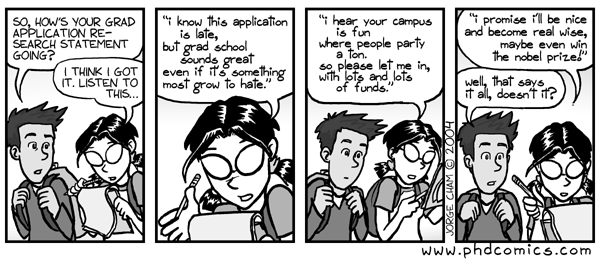
\includegraphics[scale=0.4]{files/c2.png}
\end{center}

While you might not have control over LORs (\autoref{sec:lor}) or where your go to school (\autoref{sec:your-school}), you do over your
statement of purpose (SOP) or personal statement\footnote{Few schools separate these documents and ask you to write both: SOP, which focuses on research experiences, and personal statement, which is everything more personal, e.g., why PhD, challenges, diversity, etc}! So write it well because it could make a big difference.

In your statement, you have the opportunity to connect directly with us and make your application stand out and unique. Your SOP can convince adcom members that you would \emph{fit} the program, even if you don't have very strong research experience.
A well-written SOP also shows that you can communicate, which is very important in research, and that you can effectively teach and communicate with students, which is important for TA funding (see \autoref{sec:funding}).
% is important because if you need (GTA) funding, it will provide evidence
% that you can teach and communicate with students.

There are various guides on writing SOP , and \href{https://cs-sop.org/}{many example statements} are available. In short, focus on your research motivation and convince us that you can achieve it through your experience, e.g., published papers. You should also back up your claims with concrete evidence. For example, if you say you have experience with teaching, then show what you did, e.g., undergrad TA or mentoring someone.  If you say you work on project X, then show some results (paper submitted (or even rejected), achieved X\% performance improvement over ..). Also, do not use more than 2 pages (you can have references on the third page).

You should talk about things that adcom members might not know about and can help make you \textbf{stand out} in the application pool of  thousands of applicants, e.g., you are member of a minority or LGBTQ+ group (\autoref{sec:urm}), your personal Github project with hundreds of stars or your regular contributions to well-known open-source projects (see \autoref{sec:improve-your-chance} for increasing your admission chance).


This is something easy to do, but is neglected by many
applicants: \textbf{customize the statement} for the school you're applying to,
e.g., why do you apply \emph{here}? provide names of professors who you're interested in (if they are not already in the adcom, your application might get forwarded to them for evaluation; and they might be interested in interviewing and recruiting you).
This shows that you're serious and have done homework on places you're applying to.
Adcom will look for this part (\autoref{sec:why-rejected}), so do not skip it.

Finally, you should get your SOP reviewed by your LoR writers, professors (especially those who have served in adcom), or even postdocs or PhD students (because they have been through this process).

\begin{commentbox}[Vu:]
  I often read LORs and SOP first. If I am
  persuaded by then, I would skim over other factors and advocate for
  admission (unless I see red flags in other parts). However, if I am not
  convinced, then I will likely recommend rejection (unless I see
  something really standout in other parts).
  \tcblower
  Do careful research on professors, don't mention \emph{emeritus} or adjunct faculty (see more about various types of faculty in \autoref{sec:faculty-types}).
  Also, be careful not to send statements to the wrong schools or mix
  facts (e.g., talking about school X but mentioning working with
  profs. at school Y; and do not talk about George Washington when applying to George Mason). I have seen such statements more times than I should.
\end{commentbox}



\subsection*{Additional Resources}
\begin{itemize}
    \item \href{https://chrisblattman.com/blog/2022/01/11/}{Writing your statement of purpose} by Chris Blattman
  \item \href{http://www.pl-enthusiast.net/2022/10/03/how-to-write-a-grad-school-personal-statement/}{How to Write a Grad School Personal Statement} by Mike Hicks
  \item     \href{https://cs-sop.notion.site/cs-sop/CS-PhD-Statements-of-Purpose-df39955313834889b7ac5411c37b958d?p=f5d5980a71524ebaa4e6ae57266b847c&pm=s}{CS PhD SOP database} by cs-sop.org
\end{itemize}
% \subsection{Outline of a LOR}\label{sec:lor-outline}


\section{Research Experiences}\label{sec:research-experiences}

This section discusses various research experiences that can strengthen your application.
\autoref{sec:research-opportunities} provides more information on how to find research opportunities (e.g., during your undergrad study).

\paragraph{Publications} A concrete evidence of research ability is having \emph{papers in reputable international journals or conferences}.
Having published papers, especially at top venues, is a sign that the applicant has been successfully involved in research.  Applicants admitted to top schools often have multiple first-authored papers at top places.

\begin{commentbox}[Vu:]
  Many international students mention Scopus Q1, which consists of various journals from IEEE, Elsevier, and many other publishers.  I don't know/recognize many of the journals listed in Scopus Q1. This might be something to be mindful of, as \textbf{CS} faculty might not be too familiar with Scopus or journals listed there, so devote some part in your statement to discuss the significance of your papers.
\end{commentbox}

However, it is understandable that many students do not have the opportunity to publish papers. Thus, general writings, even those under submissions or rejected, would still be good (much better than nothing).  Be sure to upload your papers with your application and talk about them in your statement (see \autoref{sec:research-statement}).  Note that local conferences and non-English journals or conferences do
not carry as much weight since their quality is often unknown to US faculty. However, if you have published in such places, you should still upload them, mention them in your statement, and explain why they are good.

% In CS, conferences are important and top conferences are prestigious. You can find top CS conferences at places such as \href{https://csrankings.org}{CSRankings}, which ranks CS programs based on how their faculty publish at top \emph{conferences} (see more in \autoref{sec:ranking}).



\begin{commentbox}[Craig:]
  GMU and many other universities allow you to upload your published papers and other writing samples. In many cases, even if the papers were not published at top places, we can still determine their quality by simply skimming over the paper.
\end{commentbox}

\paragraph{Work Experiences} Work experiences at \emph{well-known research laboratories}, such as Microsoft Research, can strengthen your
application.  Unfortunately, many good research places in your countries, e.g., VinAI in Vietnam, remain relatively unknown to most universities in the US. So you or your LoR writers should explicitly say something about them in your statement.


\begin{commentbox}[Hung:]
  The reputation of VinAI has been increasing steadily over the past few years; many of my colleagues heard about VinAI.
\end{commentbox}

\paragraph{Competitions} Winning \emph{internationally recognized competitions} can also demonstrate your research potential.
For example, participating in Math Olympiads if you want to do theory or winning ACM programming contests if you want to ``build'' systems, e.g., software analysis.

\begin{commentbox}[Thanh:]
  Due to academic culture, professors in Vietnam usually aim for (international) journals instead of conferences. Could you give some tips on how to know whether a journal is good (CSrankings, unfortunately, only consider conferences)?
  \tcblower
  Vu: One way is looking at what well-known researchers publish. For example, if you are interested in a field X, you can use CSRankings to look at active faculty in X, and then look at their websites to see what journals they publish at.
\end{commentbox}


\section{Your School and Grades}\label{sec:your-school}

\paragraph{School} Graduating from top universities \emph{that we recognize} helps. For example, if you are an international student and your school is well-known, then it is \emph{``top foreign''}, which is a plus.
However, if we do not know much about schools in your country, then we are uncertain about the quality of your school and likely treat your school as \emph{``unknown foreign''}, which can be a minus point.


\textbf{Advice}: If your school is the top in your country but you think it might not be well-known internationally, you should talk about it in your SOP (and also ask your LOR writer to do that). Of course, if you're interested in working with Vietnamese, consider  \href{https://github.com/dynaroars/dynaroars.github.io/wiki/Viet-CS-Profs-US}{CS programs in the US that have Vietnamese professors}. %It might also be helpful to have your CS dept to put itself on CSRankings so that others know about the dept, its faculty, and research.

\begin{commentbox}[Vu:]
  Sometimes PhD adcom in the US will share a document such as \href{https://github.com/dynaroars/dynaroars.github.io/wiki/Foreign-Top-Schools}{this one}, which lists the top schools in several countries. We also ask other faculty and students if we think they know about the place.  For example, when I was a postdoc at UMD, members of their CS PhD adcom asked me to evaluate applicants from Vietnam.  During my time at UNL and now here at GMU, I have looked at Vietnamese applications (whether they are assigned to me or not) and provided input to their reviewers, e.g., X is the top tech school in Vietnam and so it should be \emph{top} instead of \emph{unknown} foreign, which makes a huge difference.
\end{commentbox}
\begin{commentbox}[Deepak:]
  If an applicant is anxious about their school not being known outside their country, they can provide information about their school and department, with independent sources where such information can be verified.
\end{commentbox}

\paragraph{Grades} Having a good GPA is good. However if your school is not well-known, having top grades or rankings
usually will not help because we cannot evaluate them.  This can be an issue for students in many top international universities where the competition is so high that very good students can still have low rankings from these schools (and be overlooked by adcom).

\textbf{Advice}: As with school reputation, you and your LoR writers can mention the grading system of your university if you think that is helpful for adcom to evaluate.
Note that while having good grades might not help much,
having bad grades (e.g., < 3.0) will be \red{red flag} (unless your LORs or
statement give a proper explanation). This is especially true if you
have bad grades in relevant courses, e.g., Math and CS.

\begin{commentbox}[Thanh:]
  Vietnamese universities typically offer specialized programs, such as the talented engineer program at HUST, that have highly competitive entrance exams and a limited number of available slots (e.g., 30 per year). However, these programs often set higher requirements for students, including more demanding tests and assignments, resulting in lower GPAs and overall rankings. For example, a 3.5 GPA students from such talented programs are typically much better than a 4.0 GPA students not in those programs.  Similarly, variations in GPA standards exist among different universities, with technical universities generally having lower GPAs than economical universities. These make gaining admission in the US difficult as US faculty are not familiar with these issues.
  \tcblower
  \textbf{Vu}: Vietnamese students and even faculty often lament how this grading system hurts Vietnamese students applying abroad. One way to mitigate this is making these issues known in your SOP.  \href{https://github.com/dynaroars/dynaroars.github.io/wiki/Viet-CS-Profs-US}{Universities with Vietnamese profs} are probably aware of them, but in general your letter writers \emph{and} you can explicitly mention these in their letters and your statement.
\end{commentbox}

\section{Standard Tests (GRE, IELTS, etc), Work Experiences, Online Courses, and Certificates}\label{sec:standard-tests}


\paragraph{GRE} While a few schools still require taking the GRE (e.g., UCF), most good CS PhD programs in the US \textbf{no longer} require it.

\textbf{Advice}: If you haven't taken the GRE or have bad scores, then don't waste time (re)taking it.  However, if you took it and have really good scores then you can include and talk about them in your application (but don't expect them to make much difference). But if your scores are bad, then you should not include them in your application, which can be a \red{red flag}.

\paragraph{English Tests} Unless your degrees are from specific countries such as \href{https://github.com/dynaroars/dynaroars.github.io/wiki/About-GMU#standard-tests-waiver-eligible-countries}{these}, you will need to
take standardized English tests.

\textbf{Advice}: Just do well enough to pass the minimum requirement set by the university. %, which is required for TA (\autoref{sec:funding}). 
Just as with grades (\autoref{sec:your-school}) and GRE, having high scores in these tests might not help, but having too low scores can be a \red{red flag} and sometimes results in an automatic rejection (\autoref{sec:why-rejected}), e.g., below the minimum requirement.


\begin{commentbox}[Vu:]
  The minimum for GMU (being above this might not mean much, but below is a \red{red flag}).
  \begin{itemize}
    \item GPA: $\ge 3.0$ in your undergrad (but we also consider the rank/prestige of your school)
    \item GRE: not required
    % \item but if you want to use it, then we expect a total (V+Q) of $\ge 311$ (with a $\ge 157$ Q) and A $\ge 3.0-3.5$.
    \item English requirement tests (one of the below)
          \begin{itemize}
            \item TOEFL: 88 pts in total AND $\ge 20$ points in each subsection OR
            \item IELTS: $\ge 6.5$ OR
            \item DuoLingo Graduate English: $\ge 120$ OR
            \item Pearson Test of Academic English: $\ge 67$
          \end{itemize}
  \end{itemize}
\end{commentbox}

\paragraph{Work Experiences} Work experiences, especially if they are not research-based, \emph{do not} carry much weight. Similarly, LoR from your supervisor for non-research experience will not count much.

\textbf{Advice}: do not spend much time talking about non-research-related job in your SOP.
However, if you have research-based work experiences, then they can be useful and should be mentioned in your SOP and LORs. For example, if you have worked at a research lab, e.g., Microsoft, DoE, VinAI in Vietnam, etc (\autoref{sec:research-experiences}), then you should mention that in your SOP and ask your supervisor to write about your research experiences and potential in their LOR (\autoref{sec:lor}).

\paragraph{Online Courses and Certificates}
In general, these do not carry much weight as they do not show research ability. We do not care much if you have taken on online Coursera AI course or have a professional certificate from Microsoft.
However, as mentioned in \autoref{sec:non-stem}, if you do not have a CS background, you might be able to use these to show you have sufficient CS knowledge.

\section{CV/Resume}
The CV/Resume provides a summary of the applicant's achievements.

\textbf{Advice}: Prepare your CV in such away that it allows the reviewers to quickly scan to identify major achievements, e.g., Publications, Programming Competition Awards, and Teaching Experience.

\section{Interview and the Waiting Game}\label{sec:interview}

After you submit your applications, the waiting game begins! For many students, this is a very stressful time. This section provides some information and tips to help you get through this time.

\paragraph{Interviews} Just like a job application, you likely will get interviews from schools. The most common case is that a prof. is interested in working with you and wants to chat to make a decision, e.g., to offer RA (\autoref{sec:ra})). In some cases, the interview is done by several professors, e.g., to see if a student fits in their group or to recruit a very strong student to their program. The interview can also be done by adcom members to see if the student fits their program.
%The professor might include one of their current students as part of the interview.

Typically, an interview takes about 15--30 minutes, and one important aspect of evaluation is your ability to effectively communicate, including speaking and understanding English. 
You might be asked to talk about your research experiences and interests and to read a paper and discuss it. In some rare cases you might also be asked to solve a problem, e.g., a coding problem. 
The interview is also a good opportunity for you to ask questions about the program and the university.

\textbf{Advice}: Treat the interview as an informal chat. Have elevator pitches about your research experiences and interests. You might also want to have a 5-minute presentation about your research. If a prof. asks you to read a paper, do it and be prepared to discuss it. You can also ask if you need to prepare for a coding problem. Finally, prepare some thoughtful questions to ask, e.g., about the program, the university, or the professor's research.

\begin{commentbox}[Vu:]
  At GMU, faculty are encouraged to interview candidates. For very strong candidates, the interview is actually to recruit them.  In some cases a faculty interviews a candidate that they see potential and want to advocate for their admission. Without the interview, such applications may be more likely to be rejected.
  \tcblower
  In short, getting an interview is a good sign; it means that someone is considering you. If we are not interested in your application, we will not proceed with an interview.
\end{commentbox}

\paragraph{Follow-Up Emails} If you had an interview and have not heard back, you can email to ask about the status of your application. See \autoref{sec:accept-postpone-decline} for how to check status and follow-up emails.

\paragraph{Timeline} The timeline for interviews and notification letters varies.  Faculty setup interviews based on their (busy) schedule. Do not be surprised if you get an interview invitation in the last minute. Some schools do not do interviews at all.

Some schools send out admission letters in batches, some do rolling admission, and some do not send anything out (e.g., you're on their waitlist, or they might not send rejection letters).  In general, you should hear back from most schools by mid-March (but some schools might take longer!).

In short, there is not much you can do about this other than to be patient and wait. Also do not send emails asking about interviews or status (unless you have interviewed specifically with someone then you can ask that person for status updates and others \autoref{sec:accept-postpone-decline}).

\paragraph{Updating your profile} You should not send emails to update your profile.  However, if you have new publications or other big achievements, you can ask to update your application (though no guarantee that they will consider them).

\paragraph{Not getting interviews} While it is generally good to get an interview, not getting one \emph{does not} mean you're out.  Many programs do not have the tradition of interviewing applicants. For example, at GMU, most of our admitted students with TA (\autoref{sec:ta}) do not go through interviews.

However, no interviews typically means that you will not likely get an RA (\autoref{sec:ra}), which is offered by an individual faculty (if they you to do research for them, then they likely will interview you first).  In the case of no interviews, your application (and TA/fellowship funding) is decided by the adcom.

% \section{Preparing and Tracking Applications}


% \paragraph{Shared Spreadsheet} Many students use a (shared) spreadsheet, e.g., Google Sheets/Docs, to help them and their letter writers to keep track of their applications. Here are some information to put on the sheet.
% \begin{itemize}
%   \item \textbf{Your info}: Full name, email, phone, link to website/CV.  This is helpful for the writers just in case they want to quickly get some information about you.

%   \item \textbf{Applications details}: University, Dept, Application System URL, Submission Deadlines, Application Status (e.g., submitted,  rejected, wait-listed, accepted)

%   \item \textbf{LoRs}: Writer 1, Writer 2, Writer 3.  If this is a shared document, you might want to omit names and just use writer X. Under each is their status, e.g., sent/not yet/reminder needed, etc.


% \end{itemize}


% You can then share this sheet with your reference writers and remind them to submit LoRs on your behalf (see \autoref{sec:lor}). Also, you should periodically update your writers with your status; a simple note such as \emph{``I am getting interviewed by prof. X at school Y. Do you have any advice?''} can get you a lot of help.


% \paragraph{Communicating with LoR writers and People Who Support You}

% stressfull time, rely on support from others
% ask ppl to review your SOPs
% provide information for LORs, ..
%


\chapter{Getting Admitted}\label{sec:accepted}

\epigraph{``Oh... and how is education supposed to make me feel smarter? Besides, every time I learn something new, it pushes some old stuff out of my brain. Remember when I took that home wine-making course and I forgot how to drive?''}{\textsc{The Simpsons}}

By around March you should hear back from most PhD programs you applied to. If you haven't heard back, reach out via email and ask about the status of your application.
If you receive offers, congratulations!  Now you're at a different game because the schools that have admitted you will try to get you to accept them!  Important factors to consider include the reputation of schools and professors (\autoref{sec:schoolsandprofs}), and funding availability (\autoref{sec:funding}). You will likely have to make your decision (\autoref{sec:accept-postpone-decline}) by around \emph{April 15}, which is the deadline for most schools
(\href{https://cgsnet.org/wp-content/uploads/2024/01/CGS_April15_Resolution_Jan312024.pdf}{why this date?}).

\paragraph{Open House} Most schools have \emph{Open House} or \emph{Visit Day} events, which are a great resource to learn about the school, department, faculty, research, living, etc.
\textbf{Advice}: Even if you can't come in person, you should attend virtually and meet with individual faculty. During the event, you get a chance to learn more about the program, and talk to individual faculty and current students.  Take notes of faculty who make you excited, and count those that are taking in new students (if they meet you, likely they are considering new students!).  Talk to students about their advisers, the dept, the area, and funding situation.  Ask about anything you want to determine that they deserve \emph{you}.

\begin{commentbox}[Vu:]
  GMU has \emph{Virtual} Open House (VOH), e.g., \url{https://cs-gmu.github.io/cs-phd-voh-s23/}. We invite all admitted PhD students to the VOH through Zoom to learn about the CS program, the department, GMU, and the DC area in general. Students also get opportunities to chat with professors and current students.
\end{commentbox}

\paragraph{What else?} Make a decision, accept, reject, or defer the offers  (\autoref{sec:accept-postpone-decline}). Ask to meet with potential advisers (e.g., through Open House or separately) and even their students. Ask about computer equipment and software, office space, and other resources; in many cases these will be provided for free by your adviser or department (\autoref{sec:buying-equipment}).

Also, do not forget to update and thank your LoR writers and others who have supported you through this process.

\section{If you do not get admitted}\label{sec:not-accepted} 

If you do not get admitted to any schools or don't want to go to the ones that admit you, try again next time.  Graduate admission can involve randomness and noise. In the meantime, you can work on improving your profile, e.g., get more research experiences, publish more papers, improve your connections for better LoR writers, etc. See rejection reasons (\autoref{sec:why-rejected}) and additional advice (\autoref{sec:improve-your-chance}).

You can consider applying to MS programs, which are typically easier to get in; but you likely need to pay.  Sometimes, the university that rejected you for PhD might accept you for MS.
If you get in an MS program at a school of your choice, you can contact professors to work with them. If you do well, you can ask the professor to support you to convert to PhD.

\paragraph{Should I ask for feedback?}
No, don't bother.  You will likely not get any useful feedback.  We are not willing to reveal your evaluation results or give you advice on how to improve. So it is best to just move on.  If you really want feedback, ask your professors, collaborators, ref writers, or those who have previously applied.


\chapter{Funding}\label{sec:funding}

\epigraph{Bart, with \$10,000, we’d be millionaires! We could buy all kinds of useful things like…love!’}{\textsc{The Simpsons}}

As mentioned, if you're admitted to a \emph{good} CS PhD program, you should not have to worry about funding!
In the US, the common types of funding for PhDs are \emph{graduate teaching assistant} (GTA or TA), \emph{graduate research assistant} (GRA or RA), and \emph{Fellowship}.
RA is paid by a prof. for you to do their research. TA is paid by the department for you to help with teaching. Finally, fellowship is an independent funding that can come from a school, a company, or an organization. \autoref{tab:funding} summarizes the differences.
Note that funding is typically more available for PhD students than
Masters.

\begin{table}
  \centering
  \small
  \caption{Different types of PhD funding. All cover tuition, insurance, and stipend.}\label{tab:funding}
  \begin{tabular}{c|c|c|c}
    \toprule
    &\textbf{TA}&\textbf{RA}&\textbf{Fellowship}\\
    \midrule
    \textbf{From} & School & Profs. & School/External\\
    \textbf{For}                  & Teaching Assist.       & Research                        & Research                              \\
    \textbf{Cover All?} & Yes                      & Yes                             & Yes                                   \\
    \textbf{Summer?}              & No                       & Maybe                           & Likely                                   \\
    \midrule
    \textbf{Pros}                 & Research Freedom         & Get to do research              & Research Freedom                      \\
    \textbf{Cons}                 & Teaching Duties           & Research Restriction & Competitive, Limited             \\
    \bottomrule
  \end{tabular}
\end{table}

\section{Graduate Assistantship (TA/RA)}\label{sec:ta-ra}
The most common type of funding is \textbf{graduate assistantship}, which is either TA or RA. Both TA and RA come with tuition waiving (you don't have to pay tuition), health insurance (this takes care of your insurance, which is a must have in the US), and most importantly, your stipend (i.e., your salary). Some universities also give significant discount or pay insurance for spouse/children.

Several things about stipends.  First, the amount of stipend \emph{varies} and depends on factors such as location (e.g., a stipend in Washington DC is likely higher than in Lincoln, Nebraska due to higher living cost). Second, an academic year (AY)  year is typically \emph{9-month} in the US, so stipend is for 9 months (so divide by 9 for each month). Third, you might get paid over the summer through funding from your professor or fellowship (typically no TA over the summer). Fourth, like most source of income in the US, you will have to \emph{pay tax} on your stipend.  Finally, private universities might pay more for stipend, but they could have extra activity fee or some other hidden ones (e.g., you may need to pay some fees for each credit hour).

\paragraph{Low Stipend?} Students often complain their stipend being too low. However, in most cases it is actually not bad, and you can live comfortably with it.  It might also be enough to support your spouse and kids (many CS PhD students have their family with them). So don't worry too much about stipend.  If you're admitted to a good CS PhD program, you will be fine. A good school would know that it has to be competitive to attract students.  For example, at GMU, every year we discuss improving the benefits, and especially stipend, for our graduate students.

For a full breakdown of how much a graduate student costs, see \autoref{sec:ra-cost}.

\begin{commentbox}[Vu:]
  TA and RA at GMU have similar benefits in tuition waiving and insurance.  The college and department will set the rate for 9-month graduate assistant stipend.  TA, which is paid by the department, will likely be that amount but RA might be higher depending on the stage of the student (1st year vs ABD\footnote{All but dissertation: really close to graduate.}) and the prof.
  \tcblower
  Having health insurance is required at many US universities.  Do not assume that you're young and healthy and ignore insurance.  At GMU, and most good CS PhD programs, your GTA or GRA \emph{will always} come with full insurance. In fact, at GMU your spouse/children will get a significant discount rate for health insurance.  So you will never have to worry much about health issues for you or your family here.
\end{commentbox}


\subsection{Teaching Assistant (TA)}\label{sec:ta}

TA is common in the beginning when you haven't found an adviser who would pay you RA. It is also common to sandwich between TA and RA (e.g., when your prof. does not have sufficient funding or you want to try get TA experience).

Your TA is paid through the school or department, i.e., they hire you to help teach.
As a TA, you spend up to 20 hrs/week and help with classes (e.g., grading or teaching labs/recitation).
During a semester, a TA might work with several courses and professors (not necessarily their adviser).  TA funding is \emph{not} typically available during the summer, which has few courses.

\paragraph{How to get TA?}  Unless you have other funding such as RA or fellowships, TA is typically the default for CS PhD programs. When you apply to be a full-time student,  state that you need financial assistant. Typically, adcom will either admit you and give you GTA, or reject you; i.e., we do not admit a student without supporting them.

\begin{commentbox}[Vu:]
  At GMU CS, admitted PhD students have 4 years of GTA guaranteed, and also receive a stipend for the first summer.
\end{commentbox}

Even if you have other funding and do not need a TA, you still should do TA at least once.  This allows you to see what teaching is like, which is especially helpful for a research career where you often give talks and tell people about your work. GMU sometimes has classes that a more senior student can teach.  In that case, you will be paid as GTA or even sometimes as a lecturer.  This is a good opportunity for students to get teaching experience and also get paid more (as a lecturer).

\subsection{Research Assistant (RA)}\label{sec:ra}
RA is provided through a professor through their funding so you can work on their project.
You do not need to teach as an RA, so you can focus on your research. Depending on the professor, RA may be available during the summer. \autoref{sec:ra-cost} gives more details on RA budget.

\textbf{How to get RA?} When a professor recruits you, they might offer you an RA right away (so you start with an RA).  However, a more common scenario is that you first get admitted with TA, and then after a year or two find an adviser to support you with RA.

It is important to note that RA is \emph{never guaranteed} as it depends on the funding situation of the prof. So you should also pay attention to TA, which is a good backup plan (remember, typically TA and RA have quite similar benefits). This means you should also check if TA is readily available for PhD students in the program.


\begin{commentbox}[Vu:]
  If you got recruited an offered an RA by a prof., you will likely get admitted.  For example, if a prof., even if not in PhD adcom, wants to fund you, adcom will respect that decision and admit you (unless your application has many red flags).
\end{commentbox}

\section{Fellowships/Scholarships}\label{sec:fellowships}

Fellowship is another type of funding that students can get (e.g., from the university, industries, or government).
Fellowships are typically competitive and generous, giving pretty much all benefits tuition/insurance that a TA/RA has.  They might even give higher stipends (including summer) and open doors for job opportunities such as internships.

\textbf{How to get Fellowship?}   Many schools provide fellowships to attract students. You likely will not need to do anything and adcom will recommend such fellowships to strong students. Some schools automatically offer a fellowship to all accepted students, while others only award it to a limited number of admitted students, such as the top percentile.

For external fellowships including those from the US government (e.g., NSF, DOD) and tech companies (e.g., Google, Microsoft, Facebook), you will need to apply.  % However, tech companies including Google, Microsoft, Facebook have fellowships that international students can apply for.
Prestigious external fellowships typically require a clear and good research plan, so it might be a good idea to wait until at least your second year to have research experience and even publication before applying. Remember, you're competing with the top PhD students at top universities worldwide.

\begin{commentbox}[Vu:]
  PhD applicants at GMU are automatically eligible for a \emph{Presidential Fellowship}.  It is at least as good as GTA but the most important thing is that as a fellowship it is truly free money (i.e., you do not depend on any prof. or TA).  Adcom members nominate applicants for this fellowship and the whole committee will decide.
\end{commentbox}

In addition to general fellowships that are available to all students, there are also specific fellowships, e.g., for US citizens and permanent residents, for underrepresented minority (URM) students (\autoref{sec:urm}), and students from specific countries. There are many fellowships available, so you should look for them and apply.

In general, fellowships, especially those that are open to everyone, are highly competitive and prestigious, and you will stand out if you get one.  Every PhD student has pubs, but only a few would have NSF Graduate (GRFP) or Microsoft fellowships . In fact, these are so prestigious that even if you didn't get it but make it to the final round or even \emph{``honorable mentioning''}, school will still mention you on their website, and you should put it on your CV.

\chapter{Choosing Schools and Professors}\label{sec:schoolsandprofs}

Choosing a school and an adviser is clearly among the most important things in your mind when you apply and especially when you get admitted.  This is further complicated due to cultural differences and the unfamiliarity of international students with the US higher education system.  This section aims to mitigate some confusion and help you make informed decisions.

\section{Choosing a University}\label{sec:choosing-university}

We will first discuss universities in the US that offer PhD in CS. Then we will talk about how to select them.

\subsection{Schools that offer PhD in CS}

Most US universities have CS study, but many of them do not have a PhD program in CS. These universities might offer just Bachelor's degrees (e.g., BS) and no graduate studies (i.e., no MS or PhD degrees), or they just offer MS programs (but no PhD). For example, Penn State in University Park has PhD in CS,  but Penn State in Harrisburg only has BS and MS in CS, and Penn State in York only has BS in CS.  On the other hand, multiple locations of the University of Texas, e.g., Austin, Dallas, and Arlington, have PhDs in CS.

Thus, if your goal is PhD in CS, you have to aim only for schools offering such a degree.  %This might sound obvious but many students (even those in the US) get confused due to the large number of universities.
While this can be confusing due to the large number of universities in the US, a little research, e.g., searching for PhD in CS from the school website, will help you find out. Schools listed in \autoref{sec:ranking} have PhD programs in CS, so you can start there.

% \subsection{R1, R2, ...}

\subsection{Selecting and Ranking Schools}\label{sec:selecting-ranking-schools}
\begin{center}
  
\includegraphics[scale=0.5]{files/c1.png}
\end{center}

International students often put schools into two bins: (i) very top schools that they dream about, and (ii) everything else.  They commonly use rankings from US News, which is not transparent and questionable\footnote{\url{https://cra.org/cra-statement-us-news-world-report-rankings-computer-science-universities/}}.  Sometimes they evaluate based on the reputation of the school's undergrad program or the reputation of the school's non-CS programs such as medical, math, or physics.
They even rank universities based on popular states they know in the US, e.g., California, Texas, and New York.

You can learn about CS programs and the research interests of faculty using resources such as \href{https://csrankings.org}{CSRankings.org}. You will be very surprised to learn that a school that you didn't know much about can have very strong research in your topic (and vice versa, a school you thought highly about might have no faculty working in the research field you're interested in). This is also a good way to learn about individual faculty, e.g., who works on what, and well-known CS conferences\footnote{In CS (and probably only in CS), conferences, not journals, are often the main venue to publish research findings (see \href{https://homes.cs.washington.edu/~mernst/advice/conferences-vs-journals.html}{why here}).}. %\autoref{sec:ranking} gives the top 50 CS programs in the US according to CSRankings.

\begin{commentbox}[Dat:] Most Vietnamese students, including those from top schools, \textbf{do not know} about CSRankings.  May be applicants who worked at top research places such as VinAI would know about it.
\end{commentbox}

While many find CSRankings useful, it is not perfect, and in general, rankings are superficial, and you need to do more research to be informed and make better decisions. For example, you might prefer places with a large community from your country (e.g., Northern VA has a large population of Vietnamese). You might prefer places with high-tech companies (Seattle or Silicon Valley), with many outdoor activities (e.g., hiking, skiing), or with better weather (\emph{``PhD can be depressing, so would you rather be depressed in California or New York?''}).  You might need to think about the cost of living, e.g., living in California is more expensive than in Virginia, or places with high crime rates (note that while some university might be in a high crime city, but the campus itself is safe).

If you get admission to several places, you should consider attending Open Houses (\autoref{sec:accepted}) and contact profs. that you're interested in at those places and talk to them.  They would be more willing to chat with you now that you have been admitted.  Ask questions about \href{https://github.com/dynaroars/dynaroars.github.io/wiki/Answers-to-Ph.D-Advisor-Guide}{their work}, how they manage students, and their expectations. You can even ask to contact their students.

\begin{commentbox}[Hung:]
  I always encourage the students I admitted to talk with my students and the students of other faculty in other schools who admitted them. You will unlikely hear straight-out complaints from current students in a prof’s group. But sometimes what is important are things that they (current students) don’t tell you. Pay attention to their ``level of excitement'' being in the group.
\end{commentbox}

\begin{commentbox}[Xiaokuan:]
  Chinese students often only look at US News rankings when selecting their PhD universities (I did that, too, when I was applying for PhD positions).
  Now that I am a professor, I find it to be the least promising way.
  %
  The reason is that US News does not provide a good metric for evaluating the quality of the PhD program.
  %
  If you want to do great research, CSRankings is the best way to find good and active professors (which did not exist when I was applying),
  since it solely focuses on publications at top-tier CS conferences.
  %
  Also,
  I think PhD is not only about research;
  you need to also consider your daily life there, since you will (probably) stay for at least five years.
  %
  You might regret it if you did not consider this seriously before applying.
  %
\end{commentbox}

\section{Choosing an Adviser}
There is no one-size-fit-all answer to this question. The best adviser is the one that you can work well with.  But how do you find such a person?

Fortunately, while some non-US programs require finding an adviser and research topic before starting the PhD (\autoref{sec:non-us-differences}), CS PhD programs in the US will typically give you a couple of years to search for advisers and research topics.  This is especially true if you're admitted with TA (\autoref{sec:ta}), which gives you time to explore and find an adviser.

\subsection{Finding the right adviser}

Here is some general advice for finding a prof.  Assuming you're not familiar with any particular one, then first search for profs. that share similar research interests.  For example, in CSRankings, if you want to work with PL, you can search for those published in PL conferences.  If you want to work with SE \emph{and} AI, you can search for faculty who work in both SE and AI.  Then you research that prof. and contact them (\autoref{sec:contact}).

\begin{commentbox}[Xiaokuan:]
  Whether the student's research interest matches that of the adviser is very important;
  if there is a mismatch,
  either the student or the adviser has to make compromises,
  which often leads to disagreements or conflicts.
  IMO, the adviser should be the one who \emph{guides}  students to do research while allowing students to pursue their own interests,
  instead of \emph{dictating} their research.
\end{commentbox}


Another effective way is taking graduate-level courses in the topics you are interested in.  Profs teaching \emph{special topics courses} and \emph{research seminars} might be recruiting students---giving you even a higher chance. Do well in the class, answer questions, talk to the prof after classes, etc---being stand out.  Many profs, including myself, prefer taking in new students this way.  It gives both the prof and student more time, e.g., a whole semester, to work and evaluate the relationship before making any commitment (sounds a bit like a marriage!).

You can also ask if you can do an independent study or research with a prof. This can be informal (no credit) and takes place during the summer or winter break.  For example, I do this with multiple students, many of whom are undergrads. Many will drop out because they find they don't like my research, but some will stay and become my PhD students.

Ultimately, choose a prof. that fits you by communicating with them, taking their courses, meeting and asking them questions, and talking to their current students. It will take time and effort, but since you will be working with this person for 5+ years, it is important to try to find the right one.

\begin{commentbox}[Thanh:]
  In my opinion, having a well-suited adviser is crucial for a successful PhD and research career. One effective approach to finding a suitable professor is by working with a professor during your undergraduate studies. An exemplary instance is VinAI's residency program, where residents collaborate with professors from the US for two years before applying to PhD programs. Many VinAI residents have achieved remarkable results and gained admission to prestigious US universities. Unfortunately, VinAI's resident program is limited to AI research.

  In other fields, e.g. Software Engineering, Vietnamese students face challenges in reaching US professors. Do you have any tips for Vietnamese students who want to connect with US professors and work as research assistants?
  \tcblower
  \textbf{Vu}: \autoref{sec:contact} shows how to contact a professor for research opportunities. Many probably will say no (or do not reply) as they do not have the bandwidth to take on random students, but some may say yes if they see a potential fit.
\end{commentbox}

\subsubsection*{Additional Resources}
\begin{itemize}
  \item \href{https://www.cs.columbia.edu/wp-content/uploads/2019/03/Get-Advisor.pdf}{The Definitive ``what do I ask/look for'' in a PhD Advisor Guide}
\end{itemize}
\subsection{Types of Faculty: Who can serve as a PhD adviser?}\label{sec:faculty-types}

Not every faculty can serve as your official PhD adviser. Let's try to understand the different types of faculty and their roles. For example, you might hear about tenured,  tenure track, and teaching faculty.  You might also hear about assistant, associate, full, adjunct, emeritus, teaching, research professors. Here is a primer on these terminologies.

\paragraph{Types of Faculty} There are typically three types of faculty: tenure-line, teaching, and research.  The main difference is their focus: research, teaching, or both.  The type of faculty can affect their ability to serve as your adviser.

\textbf{Tenure-line faculty}, consisting of tenured and tenured-track profs., focus on research, which includes publishing papers, obtaining grants, and mentoring PhD students.  They often have a low teaching load (e.g., 1 per semester). \emph{Tenured} faculty are professors who have been promoted to a permanent position (informally, very hard to fire them).   \emph{Tenure-track} faculty are (more likely young) professors who are on the track to get tenure.  For most schools, tenure-line is the main type of faculty that can serve as a formal adviser of PhD students. \autoref{sec:tenure-vs-tenure-track} talks more about choosing between tenure and tenured-track professor as your adviser.

\textbf{Teaching faculty} (sometimes called instructional faculty or professor of practice) mainly focuses on teaching. They typically teach 3--4 classes per semester (which is quite a lot) and \emph{do not} have research responsibilities, e.g., they do not have to worry much about publishing papers or obtaining grants. As such they typically do not have funding (e.g., RA~\autoref{sec:funding}) to support PhD students.
Depends on the university, they might be able to \emph{co-advise} and mentor PhD students with a tenure-line faculty, but typically do not formally advise and graduate PhD students.

Note that non-CS profs (even in tenure-line ones) often cannot solely advise and graduate PhD students (see \autoref{sec:related-fields}). 

Some universities have \textbf{research faculty} or research scientists, who are typically non-tenure line faculty and focus on research (e.g., publishing papers and getting grants). 
They can recruit students and provide RA funding for them. 
They can also teach classes, but typically have a lower teaching load.
For some universities, they \emph{can} solely advise and graduate PhD students, but for others, they cannot. 

\textbf{Adjunct faculty} is not full-time, e.g., they might be working in industry and teach a class or two for fun. \textbf{Emeritus faculty} means they are retired from the university, e.g., they could move to the industry, but still have some affiliation with the university.   Due to their roles, these profs. typically do not advise PhD students.


\paragraph{Ranks} Faculty have ranks such as assistant, associate, full, regardless if they are tenure-line or teaching.  Assistant means new faculty, associate means they have been promoted, and full means they are senior. A tenure track faculty starts with being an assistant professor and then gets tenure and promoted to associate (typically after 6 years) and then full (time varies, some become full within 3-4 years, some 10+ years, some remain associate). A non-tenure track faculty, e.g., teaching or research faculty, also starts with assistant, then promoted to associated, and full prof.




\subsection{Tenured or tenure-track faculty? Who do you choose?}\label{sec:tenure-vs-tenure-track}

\begin{center}
  
\includegraphics[scale=0.4]{files/c8.png}
\end{center}


The short answer is that tenure-track faculty such as assistant professors are likely young and active in research (they have to, to get tenure). Thus, they will likely have more time to work with you and push you to do research and publish. However, they may not have as much experience in managing students and may not have as much funding (yet).

Tenured faculty, e.g., associate and full profs., are likely older, more well-known, and have more experience in managing students.  However, they might not push you as hard. They might also expect you to figure things out yourself, i.e., you need to be independent.  Some tenured faculty are also no longer active in research and are more involved with administrative responsibilities or with their startup companies (this means they will likely not take new students).

% \subsection{Strong Faculty vs High-ranked School}
% \begin{commentbox}[Thanh:]
%   When considering PhD programs, we often wonder if we should prioritize a high-ranking university or a professor with a strong reputation? Of course, both are great, but it is hard to achieve both.  I believe receiving some guidance from you  would be incredibly valuable.
% \end{commentbox}

% This is a good question and there doesn't seem to be any best answer or specific algorithm that you can use.  But I'll throw out something for you to think about. To me, there are many good schools in the US and so you have some leeway in choosing.  For example, I don't believe there's much difference among schools in top 5 (e.g., CMU, UIUC, UCSD, MIT, GTech are in the same equivalent class), top 10 (e.g., Michigan,  Stanford, UWash, UC-Berkeley, Cornell is another equivalent class), top 20, top 30, top 40, and so on (though I would say schools above 100 are pretty much in the same equivalent class).  It's hard to say a top X is much much better than a top X+20 (e.g.,  Purdue at 15 is stronger than Yale at 35, but not \emph{that much} stronger as you would think).  So keep that in mind, while ranking does matter (e.g., more active faculty, stronger students), the lower ranked universities are still pretty good, might have sub fields that are extremely strong (NCState is 40th, but in Software Engineering it is easily top 5), and many unique things.  This is in contrast with universities in Vietnam where there are large gaps among the top 5, 10, and so on.


\subsection{Should you contact a professor? How to get a desired reply?}\label{sec:contact}


\begin{center}
  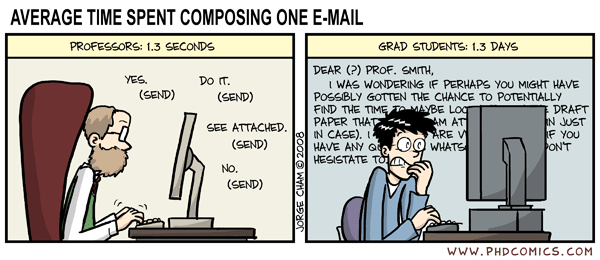
\includegraphics[scale=0.6]{files/emails.png}
\end{center}


Faculty often receive ``cold'' e-mails from prospective students. Most of the time, we ignore these emails, but in some rare occasions we do answer them. So how to write an email that gets our attention?

First, if you want to contact a prof. to \emph{ask about your admission chance}, please \textbf{don't}. We don't know and can't answer because as explained in \autoref{sec:evalapps}, we don't make individual decisions and might not even be assigned to evaluate your application.  It is the same as sending a paper draft to a journal editor and ask them if your paper has a chance.

So how to get someone to look at your profile and give input? You could ask your professors, LoR writers, collaborators, or those who have previously applied. For this kind of feedback, ask someone you have personal connection with.

On the other hand, if you want to contact a prof. to ask about \emph{research opportunities}, or \emph{GTA/GRA} support, then \emph{yes}, I believe you should---it is \emph{worth it}. However, you really need to put effort into it and do it the \emph{right way}.

First, read the prof's website, see if they say something about contacting them. Many profs. explicitly indicate how prospective students should (or should not) contact them (e.g., using specific email subjects).
In general, the best way to catch the prof.'s attention is to \emph{customize your email} for them.  For example, read their papers, know what they work on, and see if you are interested in their research. Then email them and talk about how/why their work would match yours.
In contrast, if you write a generic email that can be sent to multiple professors (e.g., if you just change some names and keywords in the email or copy and paste paper titles), you will not get a response.

Below is a good example that I would likely reply.

\begin{commentbox}[Dear Prof. Nguyen,]

  I am writing to inquire about potential research opportunities as a GRA in your group at GMU. Currently I am an undergraduate student in Computer Science at UNIV and plan to graduate in May 2023.


  I have read your TSE'21 paper on numerical invariant generation, and I am interested in this line of dynamic invariant research. I have worked (optional: with prof. Y at Z) on static program analysis and I think it could be used to tackle the spurious issues mentioned in your paper. I have a short paper at conference/workshop C and a project on symbolic execution (Github repo G).

  ...

  This is a good example because it is clearly written just for me.  It shows that the student knows about my work on invariant generation and has related  background (paper C and project G).
\end{commentbox}

Finally, profs. are very busy so don't take it personally if you don't get anything from them (though I would be very surprised if such thoughtful emails get no replies!).


\begin{commentbox}[Xiaokuan]
  Applying for PhD and contacting a potential PhD adviser is a classic \textbf{`why me, why you'} problem,
  similar to looking for a job in a company.
  On a high level,
  you need to show that you have done your \emph{homework}
  regarding the professor and the university,
  and clearly explain:
  1) why do you think you are a good fit in professor A's group?
  2) why do you want to be advised by professor A, not B?
  3) why do you want to apply for university X, not Y?
  If you don't want to spend time to do your homework,
  the chance of getting a reply is close to zero.
\end{commentbox}


\begin{commentbox}
  [Deepak:]
  In my view, cold emails are not welcome by most faculty members and should be avoided. However, if one is already admitted to a program in some department, by all means, send an email to the faculty you may be interested in working with, but do mention right at the beginning that you are already admitted to the program as well as several other universities. State specific areas (preferably specific topics-ML, robotics instead of AI).
\end{commentbox}

\subsubsection*{Additional Resources}
\begin{itemize}
  \item \href{https://yonatanbisk.com/emailing_professors.html}{A Note about Emailing Professors} by Yonatan Bisk
  \item \autoref{sec:accept-postpone-decline} How to accept/postpone/decline PhD offers (and do it gracefully)
\end{itemize}

\subsection{PhD in other related fields: CE, IST, Cybersecurity}\label{sec:related-fields}

You \emph{do not} need to do a PhD in CS to work in your area of interest. For example, in addition to a traditional CS department, GMU has IST and Cybersecurity departments, both of which have faculty with PhD in CS and work on CS topics (e.g., AI, Security, Robotics).  So it is possible that you still get to do CS research and publish in CS-focused venues even if you're not in a traditional CS program.  It is common to see faculty with CS PhD in a non-CS department as well as faculty with non-CS PhD in a CS department.

However, if your goal is a PhD in CS, then you likely need to be in the CS dept \emph{and} advised by a CS faculty. A non-CS faculty can serve in the PhD dissertation committee (common) or \emph{co-advise} (somewhat rare), but your main PhD adviser will likely be a tenure-line faculty in CS (\autoref{sec:faculty-types}). 
For example, a prof. in Stats or Math dept might be able to serve as a co-adviser, but not as a sole adviser of a student in a CS PhD program.  Similarly, a prof. in CS cannot be the sole adviser and graduate a PhD student in a Math or Stats.
If in doubt, check with the CS department for their requirements.

For this specific reason,  CSRankings includes only faculty who can advise CS PhD students. I also have compiled a \href{https://github.com/dynaroars/dynaroars.github.io/wiki/Viet-CS-Profs-US}{list} of Vietnamese faculty who can advise PhD students. \autoref{sec:faculty-types} talks more about who can serve as your PhD adviser.


\chapter{Miscs and FAQs}
\epigraph{``I want to share something with you – the three little sentences that will get you through life; number 1: Cover for me, number 2: Oh, good idea, Boss, and number 3: It was like that when I got here.''}{\textsc{The Simpsons}}

\section{Why did I get rejected?}\label{sec:why-rejected}
Many possible reasons!  Other than not having a strong profile (e.g., research potential, GPA, LoRs, SOP, poor interviews), here are some other reasons.

\paragraph{You aim too high}  This is a very common reason: you have applied to schools that are too high for your profile. While being ambitious is good, you should understand how PhD admission works (e.g., by reading this document and realizing things such as having a good GPA doesn't mean much to top programs) and be realistic! 

Before applying, you should talk to your professors and ask them to give you an honest opinion on where you should apply. You should also apply to a range of schools, including ``safety'' ones. 

\paragraph{Not a good fit}  You could have an excellent profile, but if you are interested in a research area that the program does not have, you might not be admitted.
Similarly, if there is no faculty who is willing to advise you (e.g., they are on sabbatical or personal leave, do not have sufficient funding, or already have too many students already), you will not be admitted.  This is actually good for you, as you don't want to be in a program where no one can advise you.

For example, the 2024 admission cycle has a huge surge in students interested in AI and NLP (thanks, ChatGPT!). Consequently, AI/NLP faculty might be overwhelmed and cannot consider many candidates, even those with excellent profiles.

\paragraph{Low English exam scores (e.g., IELTS or TOEFL)}  While professors might not care much about these, there might be a certain minimum set by the college or the university that you need to pass to get admitted, especially for TA funding (e.g., you need to communicate well with students as a TA).  Thus, while professors are willing to argue for your case, they might be reluctant to go against the standard requirement of the university on English scores.  Note this is for international students, as domestic ones (or those from these \href{https://github.com/dynaroars/dynaroars.github.io/wiki/About-GMU#standard-tests-waiver-eligible-countries}{countries}) do not have to take these tests.


\paragraph{Overqualified or Lack Interest}  This might be paradoxical and is the opposite of aiming too high. However if adcom believes that you are likely to get admitted and go to a better program (i.e., they are just your ``safety'' schools), they might not be so enthusiastic to admit you and want to save the spot for someone else.

A related reason is that you did not show enough interest in the program.
For example, your SOP did not mention any faculty or research area at the program, you did not respond to professors interested in interviewing you (which might be considered unprofessional and burn bridges), or during the interview you show little knowledge, interest, or enthusiasm (because they are your safety schools) in the program or profs.

\paragraph{Red flags in Your Background} Plagiarism, cheating, or other academic dishonesty are \red{red} flags. Another one is if you have a history of jumping from one program to another (e.g., you have been in multiple different programs in a short time). How would the reviewers know?  They might have contacts in other programs and heard about you, your LoRs might mention it.

If you think you have these issues, you should address them in your SOP or ask your letter writers to do so.
In general, these things are rare, but they do happen and cause concern to the adcom.


  %\item \emph{You did not make a good impression}.  For example, you might have contacted a professor and they did not like your email.  Or you might have met a professor (e.g., at a conference) and they did not like your presentation.  This is rare, but it happens.



%\section{How exactly do you evaluate an application?}\label{sec:ievaluate}

% Around 15 minutes on average (less than 10 mins for definite rejection; 20+ mins for acceptance). In earlier years I spent more time, but now I can quickly tell if an application is good or bad.

% The evaluation system allows for downloading a single pdf that consists of a summary page (e.g., schools, GPA, standard test scores), transcripts, test results, LoRs, CV, SOP, and writing samples (if any). I typically review the application in this order.  I also make notes on what I've seen, using them to support my evaluation.

% I first skim the summary for school, GPA, standard tests and look for red flags like low GPA or test scores that do not meet the minimum requirements set by the university. Then I scan transcripts for low/failing grades on CS and related courses.  For these I make comments such as ``- unknown international school with good GPA, too many low grades on CS and related courses" or ``+ very good GPA from top school XYZ". I do not look at test details as the summary already gives the main scores.

% Then I look at LoRs.  I read carefully good LoRs and quickly skim over bad or generic ones (very easy to tell, you don't even need much experience to distinguish between strong LoRs from the rest). My comments for LoRs include ``+ very strong LoRs from well-known prof. XYZ talks about research experiences'' or ``- generic LoRs, mostly about course work''.  I also note any unusual or unique details in the LoRs, e.g., ``+ LoR mentioned about student's significant contribution on well-known open-source project X''. Sometimes a LoR came directly from a GMU professor who mentioned they already know the student and intend to offer RA, which is a very strong signal for admission (and my comment would be ``Prof. X making RA offer'').

% I skim over CV, looking for paper publications, research work experiences, and other relevant achievements such as winning prizes in well-known international programming/math competitions.  My notes for CV include things such as ``+ has X papers at top venues'' or ``+ gold medal at X''. Sometimes I also note about unusual or unique experiences, e.g., ``+ has a patent on X''.

% Next is the SOP, which I read carefully (but if it is bad then it would be a quick read). My notes for SOP include things such as ``- SOP mostly on course work, no clear motivation, generic" , or ``+ very enjoyable SOP talking about XYZ, customized for GMU, mentioned profs. X,Y,Z".  If the SOP mentioned publications then I would have ``+ has X papers at top venues" or ``+/- has X papers but at unknown places''.  I will not go online to search for the papers (unless they upload them as sample papers).  I also skim over sampling papers, essentially looking over the abstract to see if reads well, and make notes such as ``+ have a paper under submission to unknown venue, but reads well". If the student mentioned a project, I might also look at it (e.g., if it is on Github) and make notes such as ``+ has project on Github with X stars''.


% At this point I have enough to make up my decision, which I enter into the evaluation system. Typically my decisions are either \emph{reject} or \emph{admit with full funding}.  For the latter, I also mention funding sources (e.g., RA from prof. X or TA). I also include my comments to support the decision. Finally, I also recommend very strong students for the University Presidential fellowship (\autoref{sec:fellowships}).

% The adcom chair will look at all evaluations for each application and make a decision (likely following the decision of the reviewers).  If there are discrepancies such as one voting reject but another full funding acceptance (such cases are rare, but do happen), the chair might ask the reviewers to coordinate to reach a consensus.

%\section{Why are rejection letters sent so late?}\label{sec:late-rejection}

%"Just reject me already!" is a common sentiment among applicants.  Indeed, school will first send out admission offers to the top candidates. They do not send out rejection letters because there is still a chance that some of the top candidates will decline the offer. If they do, then the school will go to the next set of candidates and send out offers to them.  This process continues until all spots are filled.  This is why you might not hear back until late in the admission cycle.


\section{Increasing my admission chance}\label{sec:improve-your-chance}

\begin{center}
  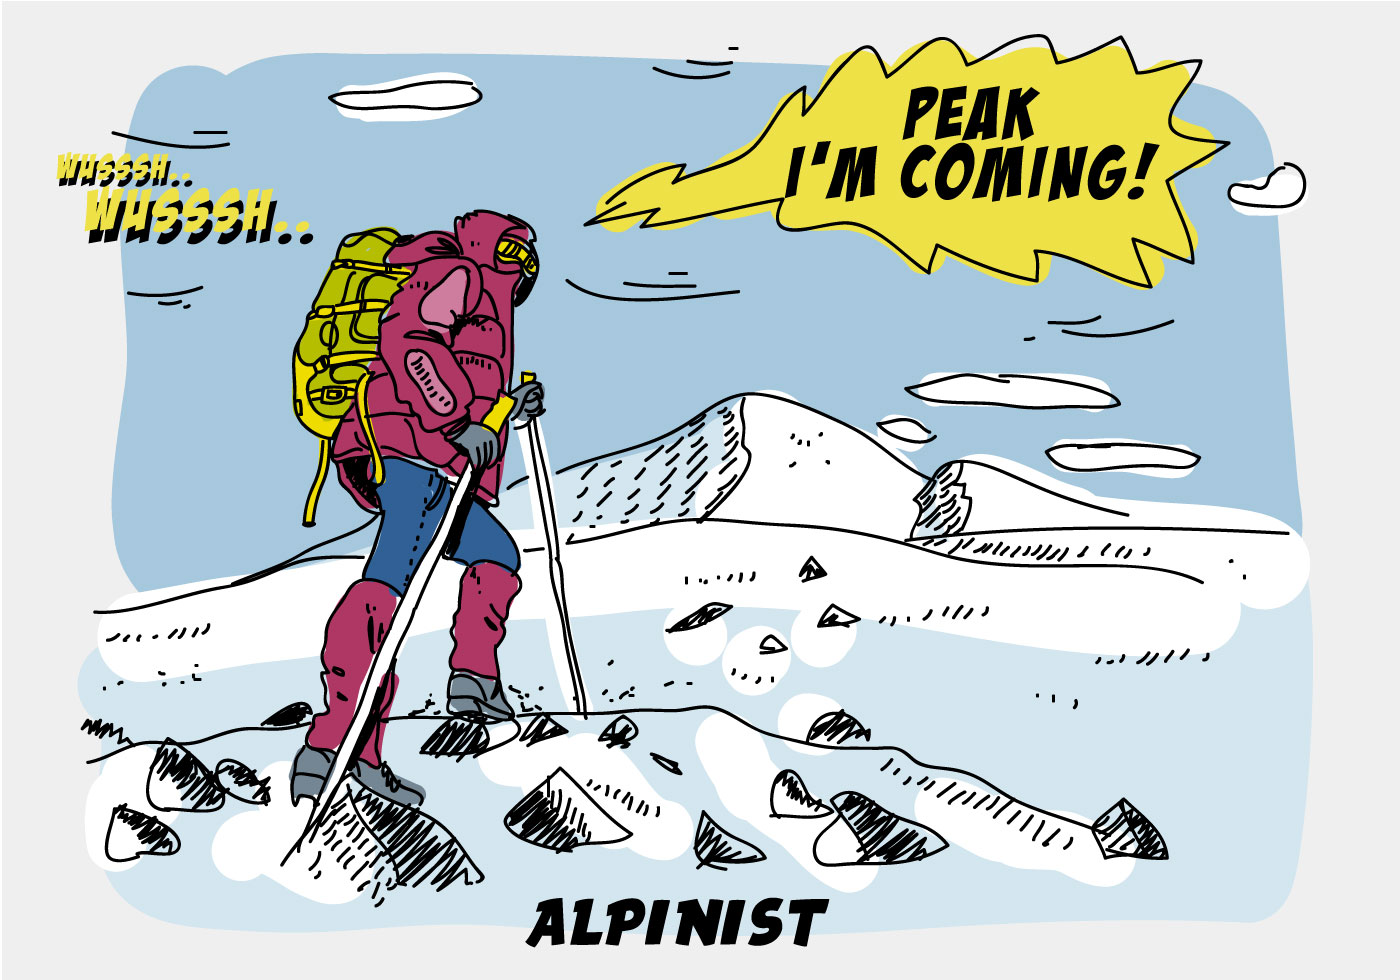
\includegraphics[scale=0.2]{files/alpinist-climbing-peak-mountain-comic-hand-drawn-vector-illustration.jpg}
\end{center}


Given the high number of quality applicants and limited number of spots, in addition to having a good application profile, you really want to show something that makes you \textbf{stand out}.  For example, even if you do not have research experience, you can talk about your personal projects, as long as they can help show you can do research. For example, if you have an open-source project on Github that is used by many people, has lots of stars in Github, do talk about it. If you often write technical, research-like blogs with many viewers, talk about them too.

There are other things you might not think are important but can make you stand out. For example, if you have a strong background in a non-CS field but can be integrated with CS, e.g., you have a degree or background in \emph{dance} or \emph{music} and want to integrate them with CS, do talk about it. Are you a female or a minority in CS (\autoref{sec:urm})? Do you participate in outreach activities that help increase diversity and inclusion in CS? Diversity is highly valued in CS programs in the US, and experiences in these areas can make you stand out and get noticed from reviewers.

\begin{commentbox}[Vu:]
In his \href{https://matt.might.net/articles/how-to-apply-and-get-in-to-graduate-school-in-science-mathematics-engineering-or-computer-science/}{post}, Matt Might was initially unsure about an application. However, upon learning that the applicant had led a 100km hike in the Himalayas, he decided to accept the applicant.  This is a good example of being \emph{stand out}, and I would also advocate for that student as this shows they have the persistence and determination required for research.
\end{commentbox}

% It is worth noting that in many cases,  an application could be rejected by most reviewers, however have a "champion", who doesn't even have to be in the Admission comittee, that strongly advocate for your profile.

\section{Member of an underrepresented or LGBTQ+ groups}\label{sec:urm}
A common question is whether you should mention that you are a member of an underrepresented and minority (URM) group\footnote{URM in CS in the US include African Americans, Hispanic Americans, American Indians/Native Alaskans, Native Hawaiians/Pacific Islanders (excluding Asian Americans), and multiracial students identifying with at least one of the previously listed URM categories.} or LGBTQ+ group (e.g., in your SOP).
This is a strong concern for international (and even domestic) students, who may have encountered discrimination in their countries or personal experiences.
%This question arises often for international (and even domestic) students. The main worry is that they might get discriminated against, as often happen in their countries or personal experiences. %, and (ii) mentioning this might make them look like they are asking for special treatment.

In my personal opinion, highlighting URM or LGBTQ+ identity can \emph{indeed be beneficial}, especially if you can articulate how your diverse experiences contribute to diversity and inclusion in academic.  Many universities have a strong commitment to diversity and inclusion and actively
\emph{recruit students from underepresentative backgrounds} (e.g., some \href{https://cse-climate.engin.umich.edu/reports/climate-dei-reports/cse-climate-and-dei-report-2022-2023/#grad-ethnicity}{stats from UMich CSE} and \href{https://www.gmu.edu/news/2022-09/mason-now-top-10-public-university-diversity-innovation-and-cybersecurity-education-us}{GMU} often promotes itself as one of the most diverse universities in the US). Moreover, many scholarships and fellowships are created specifically for URM and LGBTQ+ students, which you should explore if qualify.

It is understandable that you might feel uncomfortable disclosing this, fearing you would lost a chance of working with a faculty due to their bias.  However, if someone has this issue, then you might not want to work with them anyway (and such bias is not acceptable in academic and likely would not be tolerated by the university). In my experience, it is the opposite: \emph{many profs. actively seek out to work with students from diverse backgrounds and view diversity as an asset to their research group}.

Moreover, promoting diversity aligns with the goal of broadening participation in computing (BPC) that is strongly supported within academia (e.g., see the \href{https://plans.bpcnet.org/GeorgeMasonUniversity_ComputerScience_DepartmentalBPCPlan.pdf}{BPC plan at GMU CS}) and government funding agencies such as NSF (e.g., see \href{https://new.nsf.gov/cise/broadening-participation}{here} and \href{https://www.nsf.gov/pubs/2022/nsf22125/nsf22125.jsp}{here}).
Also, sometimes providing this information can make it easier for faculty to apply for certain scholarships or fellowships to support you, e.g., from a private donor that has offered a fellowship only to students from certain background.

Ultimately, this is a personal choice and you do what you feel comfortable.
If you do not feel comfortable disclosing this, you should not feel pressured to do so and you should also ask your LoR writers to not disclose this information.
Note that you can still talk about your experiences and perspectives without mentioning your identity.
If uncertain, you can seek additional guidance from your close professors and collaborators However, it is important to recognize that diversity is strongly valued and celebrated within CS programs in the US, and that you should feel empowered to share your unique experiences and perspectives.

%https://www.edsurge.com/news/2018-05-18-how-cornell-university-diversified-its-incoming-phd-computer-science-student-body

%https://academia.stackexchange.com/questions/130591/is-it-standard-for-us-based-universities-to-consider-the-ethnicity-of-an-applica

%https://www.cs.cornell.edu/~bindel/paper/diversity.pdf

%https://cs.brown.edu/degrees/doctoral/applications/helpful-resources-applying-computer-science-phd-programs/

\section{My undergrad was not in CS or related areas}\label{sec:non-stem}

You still can apply to PhD in CS \emph{as long as} you can demonstrate you are ready for it through your background, research experiences, LoRs, statements, etc. You might be even able to leverage this to make your profile stand out as mentioned in \autoref{sec:improve-your-chance}.

A main question adcom has for a non-CS or non-STEM student is if you have the sufficient technical background obtained through core CS courses.  So you need to show that you have such knowledge through your coursework, projects, or research.
For example, if you have taken a course on Algorithms, even online ones like Coursera, you can talk about it in your SOP.  If you have done a project that requires knowledge of OS or have a professional certification (e.g., A+) through work, you can talk about it.  If you have done research that requires knowledge of Discrete Maths, you can talk about it.  You can also ask your LoR writers to talk about your technical background.
In summary, in your application, convince us that you have the background to do CS PhD research.


\paragraph{Core CS areas} Common CS areas that you should have knowledge in are:
\begin{itemize}
  \item Programming Foundation (e.g., programming in C/C++ or Java, OOP)
  \item Discrete Math (e.g., logic, set theory, proof techniques)
  \item Data Structures and Algorithms (e.g., linked lists, trees, sorting, searching)
  \item Computer OS or Systems (e.g., memory management, file systems, processes)
\end{itemize}

In short, you \emph{do not need} to formally taking CS courses, you just need to show that you have these essential knowledge, e.g., through the mentioned ways. Many universities are well-aware that incoming graduate students might not have all the technical background, so they often have a \emph{``bridge''} courses to help students catch up.  For example, GMU has four bridge courses corresponding to the four core areas above that incoming students can take to catch up on their CS knowledge.


\begin{commentbox}[Vu:]
  I would strongly advocate for a non-STEM student who shows that they have a strong drive for CS by studying core CS knowledge through various channels (e.g., self-study through online courses, projects, etc.).  I have seen many students with non-CS background who are very successful in CS PhD.  I also have seen many students with CS background who are not successful in CS PhD.  So it is not about your background, it is about your drive and passion for CS research.
\end{commentbox}

\section{Is an MS required for admission to PhD in CS?}\label{sec:msrequirement}
No. In fact, student can get MS degree ``along the way'' to PhD, e.g., after finishing course work in the first 2 years.  However, MS can help admission if it gives research experience or is from a more well-known school than your undergrad institution (\autoref{sec:your-school}).

If you have an MS then some course work \emph{might be} transferred for course credits, which save a bit of time. But overall don't count on this, especially if your MS is not from the US.


\section{How long does to complete the CS PhD program?}\label{sec:time}


\begin{center}
  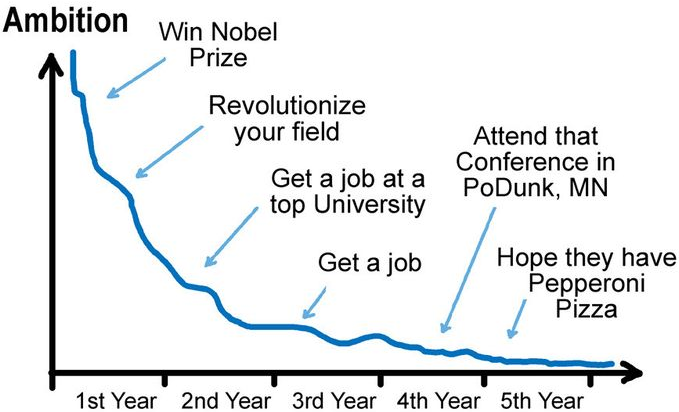
\includegraphics[scale=0.5]{files/c4a.png}
\end{center}


Typically, it takes 5--7 years for CS PhD in the US.  This can be longer than CS PhDs in other countries, which might require MS first (recall that CS PhD programs in the US do not require MS and you can get MS along the way to PhD). Within these 5--7 years, CS PhD students often take a ``leave of absence'' for 1--2 semesters to do internship at companies and research labs.

The first 2 years you typically take coursework (somewhat equivalent to an MS study), find an adviser, learn how to do research.  The next 2--3 years you focus on your research, form dissertation topic, and get results published. The last 1-2 years you continue to publish, write and defend your dissertation, and look for job.
In many cases you might take a summer or two off to do internship to get additional research opportunities.
The PhDComics figure on top shows the ``ambition'' level of a PhD student over their years of study (they miss the 6--7th year when the ambition is \emph{``Just let me graduate''}).


\section{PhD in the US vs. Other Countries}\label{sec:non-us-differences}

This summarizes the main differences between CS PhD in the US and other countries. % This is based on my experience and what I heard from others who did PhD in other countries.

\emph{MS requirement and PhD duration}:  as mentioned in \autoref{sec:msrequirement} and \autoref{sec:time}, CS PhD programs in the US do not require MS degree.  In contrast, many other countries require having an MS degree before joining a PhD program.  This means that US PhD programs are longer (5--7 years, 2 of which are coursework) than other countries (3--4 years, no coursework).

\emph{Project proposal}: in many countries, you have to choose a project and adviser \emph{during} the application process (e.g., you write a proposal to a potential adviser). You start your research right from the beginning. 

In the US, you often start your PhD without an adviser or project and find them later. You will have two initial years to explore and find an adviser and research topic. And then you often explore projects with that adviser before settling on one (can take a couple of years). 

\emph{Course work}: as mentioned above in the US you will spend the first couple of years taking classes and exploring potential adviser and research topics. 
After that, you also have to pass a series of exams during your PhD, e.g., qualifying exam, comprehensive exam, thesis proposal defense\footnote{The word ``ABD'' (all but dissertation) is used in the US to refer to a PhD candidate who have finished all course work and exams and only need to write and defend their dissertation.}.

In other countries, you start your research right away, e.g., you immediately work on the research project you proposed with the adviser you chose. Moreover, you might not have exams like those in the US or only have to do a few of them.

\emph{Funding}:  In many countries funding comes from the university or the gov't. This funding often has a fixed duration (e.g., 3 or 4 years).  In the US (\autoref{sec:funding}), funding (e.g., RA) comes directly from your adviser (no fixed duration).  There are also fewer TA opportunities in European universities compared to the US.

\emph{Academic position after PhD}: In other countries, PhD graduates interested in academia typically apply for additional research appointments, i.e., postdocs, and then consider faculty positions. 

In the US, PhD graduates often apply directly for faculty positions (postdoc for US graduates is no longer a popular option as it was before).

\emph{Work-life balance}: PhD students in the US are often said to be overworked compared to other countries, e.g., in Europe.  This is partly due to the longer PhD program and that US PhD students are often paid through TA, which requires them to do TA in addition to their own research. In contrast, PhD students in other countries are often paid through fellowships, which might not require doing TA.



\section{How do I call or address a professor?}\label{sec:address}

\begin{center}
  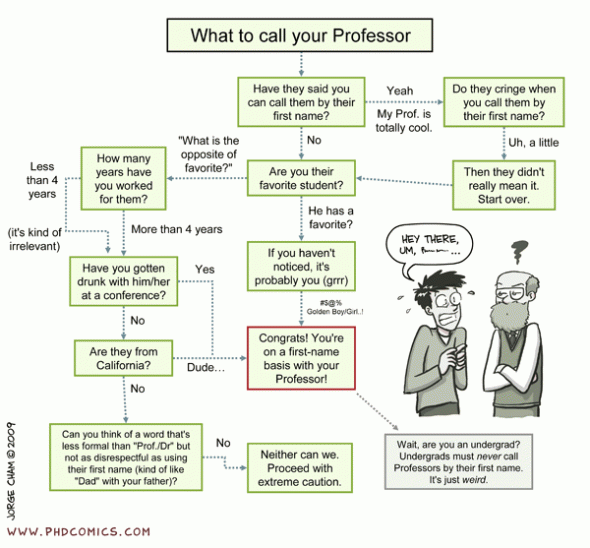
\includegraphics[scale=0.5]{files/c5.png}
\end{center}

If you're reaching out to a professor for the first time,  address them as Prof. or Dr. Lastname. Many international students use Prof. or Dr. FirstName LastName, but this can come across as if you're simply copying and pasting names. It's not necessary, so stick with Prof. or Dr. Lastname.


Furthermore, avoid using Mr. or Mrs., or the professor's first name if you're not acquainted with them yet.  As you become more familiar with your prof and depending on their preferences, you may transition to addressing them by their first name.
For example, I prefer that my students and colleague call me Vu. Some students call me \emph{Dr. Vu}, which I find a bit amusing but am totally fine with it.

\begin{commentbox}[DK:]
  I was amused to read this as if I recall correctly, you never called me by my first name when you were at UNM. You always called me Prof. And, many times, I would jokingly call you back as Prof. Vu.
  \tcblower
  \textbf{Vu}: Yes, for some reason I enjoy addressing you as ``Prof.'' (without appending a last or first name).  The use of Prof. Vu may have foreshadowed my future in academia.
\end{commentbox}

Note that in some universities the formal title Dr. Lastname is preferred over Prof. You just need to observe and follow the conventions at your particular institution. Additionally, be aware that not all faculty members may hold a PhD, in which case using Prof. Lastname is a suitable alternative.


\paragraph{Referring to professors you know} Because you are already familiar with these individuals, you can just informally use their names if they are OK with it as mentioned above (or Dr./Prof., if you want to be formal). You can also include their institution if it makes it more precise.  For example, I can say:  \emph{``I did my postdoc with Jeff Foster at Univ. of Maryland''}.

Do not include ranking (e.g., Assistant, Associate, Scientist, ...) when referring to someone. I see many international students include a lengthy title of people they know, e.g., \emph{I am advised by Asst. Prof. X, and I also collaborate with Distinguished Scientist Y}.  This is \emph{not necessary} and makes it look like you're trying to show off your connections. These nuances represent some cultural differences that you may encounter and will gradually adapt to. More on cultural differences in \autoref{sec:cultural}.

\section{How much do \emph{I} cost?}\label{sec:ra-cost}

PhD students often ask why their salary is so low compared to ludicrous grants their advisers get. They also wonder why their offer letters sometimes show that their benefits higher than what they actually receive (i.e., stipend).

\begin{center}
  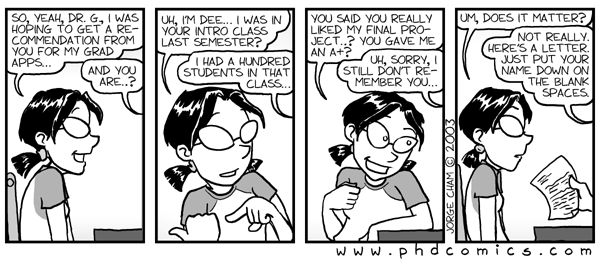
\includegraphics[scale=0.3]{files/c6.png}
\end{center}

\begin{table}
  \centering
  \small
  \caption{GRA cost breakdown. F \& A is Facilities \& Administrative Cost Base and
    MTDC is Modified Total Direct Cost. These are things that the university can charge overhead to.}\label{tab:cost}
  \begin{tabular}{rcl}
    \textbf{Budget} & \textbf{Cost \$} & \textbf{Notes} \\
    \midrule
    GRA (9-month) & 29K & \\
    GRA (summer)  &10	& 3-month, 20hrs/week\\
    \textbf{Total Salary} &\red{39K}	&\\
    \midrule
    Health Insurance	&3K	& full year\\
    Tuition (In-State) &	15K	& (\$680/ Credit + \$150/Student Fee/ Credit)* 9 credits = \\
                    &&\$7470 (\$6120 + \$1350) per semester\\
    \textbf{Total Tuition \& Insurance}	&\red{18K}	&Full year tuition + insurance\\
    \midrule
    Conference Registration	& 500 & \\
    International Travel &	1800& \\
    Domestic Travel	& 700	& \\
    \textbf{Total Travel}&	\red{3K}	\\
    \midrule
    Total Direct Cost	& \red{60}	&Salary + Travel + Health + Tuition \\
    F \& A (MTDC)	& 21K	& Direct Cost - GRA Salary\\
    Total Indirect Cost	& \red{12K}	&58.9\% of MTDC\\
    \textbf{Total (Direct + Indirect)} &	\red{72K}	& Budget for a GRA\\
    \bottomrule
  \end{tabular}
\end{table}

\autoref{tab:cost} shows the budget breakdown for a GRA per year.
These numbers are based on my experience at public universities in the US. Private universities may have different numbers.  For simplicity, I will assume the department has a 9-month stipend of \$29000 and a 3-month summer of \$10000 (about a third of the 9-month stipend). I will also use GMU tuition rate of about \$15,000/year for full-time study (which is quite cheap compared to private universities, e.g., Univ. of Chicago is a whooping \$70K) and a 58.9\% rate on \emph{indirect cost}, which is a typical rate charged for overhead or administrative costs (yes, after all, universities are businesses!).  Finally, I assume the students take two conference trips per year, one domestic and one international (conf. registration, airline tickets, taxi, meals, etc are all included).

At the end, the total budget comes out to be \$72K/year to support a PhD student. \emph{The summary is that over your 5--6 years of your PhD, you cost about \$400K, and while your stipend is X, your adviser probably pays 2X for you}. But of course the nicest thing is that you do not have to pay for any of this! You get to gain the knowledge, do research, travel, (and don't even have to buy any research or computer equipments as mentioned in \autoref{sec:buying-equipment}) and also get paid!

% \section{Having fun during a PhD?}
% PhD students \emph{and faculty} probably find it amusing about the notion that students, especially international ones, can genuinely enjoy their PhD studies. In fact, after reading posts after posts on VietPhD.org on how PhD students are commonly mistreated, stressed, it seems being miserable is a norm during a PhD study.

% There are many advice on surviving PhD that you can follow. But here I just list a few that works for me and what I advice my students to do.\tvn{TODO}


\section{Buying Computer Equipment}\label{sec:buying-equipment}

Understandably students get excited about their upcoming PhD journey and want to buy new computer equipment and electronics to prepare. However, you should check with your adviser first.  They might have funding to buy you computers and other equipment (e.g., software, books, keyboards, headphones, tablets, etc). Many CS programs also provide some budget or computer equipment to incoming PhD students (e.g., a laptop).

\section{Can I negotiate my PhD offer (e.g., if I have multiple offers)?}\label{sec:negotiate}

For stipend, unlikely for TA, which is set by the university. Moreover, while RA is set by the adviser, it is often based on the department's standard, and it also would be unfair to other students if you get more.  However, your stipend is often increased every year (automatically by a small amount) and also after you pass your qualifier exams.

For start date or TA assignment (e.g., TA'ing a specific course), it is uncommon but you can ask for it. Also, there is typically no moving allowance for PhD students. In short, standard things set by the university or department are unlikely non-negotiable.  However, you can ask for things such as computer equipment (\autoref{sec:buying-equipment}), books, (and sometimes even furniture), and a conference travel budget.


\section{Will I be miserable during my a PhD?}\label{sec:happy}
There are many stories on how students are mistreated, stressed, and miserable. Issues including bad relationships with professors, conflicts with co-authors and lab mates, feeling discriminated (e.g., because you're an international student), etc \emph{do} exist, and it is good to be aware of those.  However, in reality there are many good mentors, supportive lab mates and department, and so on.  So don't let social media make you feel pessimistic and deter your quest to advance knowledge.

\appendix



% \section{Additional Resources}
% \begin{itemize}
%   \item \bibentry{nlpphd}
% \end{itemize}

% \chapter{Additional Resources}


% \chapter{Undergraduate Research Opportunities}

% Prospective PhD students are often unaware of the importance of research experience in their application.  This provides both concrete research experiences and potential LOR writers that can talk about your research ability.
% % This is especially true for students from small colleges where research opportunities are limited.
% This section aims to provide some guidance on how to gain research experience as an undergraduate student. %This section is written together Didier, a PhD student at GMU who did his undergraduate study in Rwanda.

% \paragraph{Locally} There are many ways to find research opportunities right in your own institution.  If you did well or like a class, you can check with the professor of that class for research opportunities.  Sometimes professors would mention that they look for undergraduates on their websites, so do check those out! Even if they say they are looking for graduate students, you still should contact them and ask.  You can also ask your academic adviser or other faculty members for suggestions.  Finally, you can also ask your peers who are already doing research.  You can use the method described in \autoref{sec:contact} to contact professors

% In short, the most important thing is that you need to \emph{ask}!  Don't be shy, don't be afraid of rejection, and don't be afraid of being ignored or that you're not good enough.  Just ask!  The worst thing that can happen is that you get a ``no'' or no response.  But you will never know if you don't ask.  And if you get a ``no'', you can always ask again later.  There are students who got rejected the first time but got accepted the second time.  So don't give up!

% \paragraph{Online Research Communities and Open Source Contributions}:
% Places such as Github offer many opportunities for research, even though they might not appear so (e.g., they do not explicitly mention research). Students can explore repositories related to their areas of interest, collaborate with other contributors, and actively engage in open source research projects. By contributing code, fixing bugs, implementing new features, or providing documentation, students can gain practical research experience and interact with experienced developers and researchers in the field.

% \paragraph{Paid or Unpaid}  travel opportunities, publishing opportunities, etc


% \section{Virtual Research Opportunities Beyond Physical Boundaries (written by Didier)}
% \didi{In my experience, prospective PhD students (from Rwanda) are often unaware of the information provided in this document throughout their undergraduate. For this reason they often find themselves unprepared for PhD admission process by the time they finish undergraduate and have to spend a year or more to improve their application profiles. I think it would be beneficial to expand the document to also target students who are not yet ready for the application process to help them improve on all criteria considered during admission. I drafted the short essay on how to gain research experience remotely in order to improve their research profile and potentially get LOR from experts (hopefully faculty)}\\
% In the realm of computer science, research experience plays a crucial role in securing admissions to top-tier PhD programs. However, students from underrepresented small colleges, both in the United States and internationally, often encounter limited research opportunities within their institutions. Thankfully, there exists an alternative pathway for these aspiring researchers to gain valuable research experience, even without being physically present at a university.

% \textbf{Virtual Research Programs}:
% Several universities, organizations, and research institutions offer virtual internships and research programs aimed at providing hands-on research experience. These programs often involve working remotely under the guidance of experienced mentors and collaborating with a team of fellow researchers. For instance, \href{https://docs.google.com/forms/d/1btIwt4HwjyKMOUk-EMy3rbkfWzFxv2lNrMm_zkd0pA4/viewform?edit_requested=true}{UIUC+ Summer Undergraduate Research in Software Engineering}  offers an unpaid remote internship for software engineering students all over the world to collaborate with mentors from University of Illinois at Urbana Champaign.
% Virtual internships offer opportunities to contribute to ongoing research projects, conduct experiments, analyze data, and write research reports. Students can search for such programs through university websites, research institutes, or as of recently chatGPT (or Bard).



% \textbf{Online Conferences and Workshops}:
% Attending online conferences and workshops is another way to gain exposure to cutting-edge research and establish connections with experts in the field. Many conferences now provide virtual participation options, enabling students to access research talks, poster sessions, and panel discussions and sometimes access designated chat rooms or networking events where participants can engage with researchers, ask questions, and seek potential research collaborations. It is beneficial to also create profiles academic collaboration platforms such as ResearchGate. By creating profiles, joining relevant research groups, and participating in discussions, students can connect with established researchers, contribute to ongoing projects, and potentially collaborate on publications or research proposals as they provide access

% In conclusion, for students lacking research opportunities at their small colleges, the virtual realm offers a wealth of possibilities to gain valuable research experience. Engaging with open source projects, joining online research communities, utilizing academic collaboration platforms, participating in virtual internships, and attending online conferences are all avenues to contribute to research, connect with experts, and enhance one's research profile.

\chapter{Domestic Students}\label{sec:domestic-students}

Most of what is written in this document is applicable to both domestic\footnote{For simplicity domestic means you did your undergrad (or MS) at a US university.} and international students.  However, there are some differences and benefits that domestic students should be aware of.

\paragraph{Standing out \autoref{sec:improve-your-chance}} There are \emph{few} domestic applications compared to international ones, i.e., domestic students are minority (\autoref{sec:urm}) in the CS PhD application pool. Many US universities want to increase the number of domestic students in their programs (and as mentioned above, there are specific fellowships for domestic students).
That makes you stand out and can help your case.

\paragraph{Fee Waiving} Some school might offer application fee waiver for domestic students.  You should check with the school you're applying to.

\paragraph{School \autoref{sec:your-school}} We already know about your school, which is a plus (see \autoref{sec:your-school}). You are also more familiar with the US education system and culture (so hopefully you are aware of the cultural issues listed in \autoref{sec:cultural}).

\paragraph{Standard Tests \autoref{sec:standard-tests}} You do not need to take TOEFL or IELTS because you already did your undergrad (or MS) at a US university.  You might also be more comfortable communicating in English, e.g., contacting professors (\autoref{sec:contact}).

\paragraph{Transcripts} You do not need to get your transcripts evaluated/translated (which can be a hassle and inaccurate).  You can just send your official transcripts directly to the school you're applying to.

\paragraph{Funding \autoref{sec:funding}} You have more opportunities for funding, e.g., through government scholarships for US citizens and permanent residents.  You can also apply to specific programs \emph{before} you start your PhD, e.g., NSF Graduate Research Fellowship Program (GRFP) and Hertz Foundation Fellowship.  These fellowships are very competitive and can significantly improve your admission chance if you get them.

\paragraph{Research Experiences \autoref{sec:research-opportunities}} You might have many opportunities to do research as an undergraduates, e.g., through REUs and internships at your undergrad university.  Highlight such experiences in your application.

\paragraph{Open House \autoref{sec:accepted}} It is easier for you to attend open house events in person.  This can help you make a better decision on which school to attend.

% \begin{domesticbox}[Domestic students:] If you're a domestic student, you have several advantages in your application.   You also have more opportunities for funding, e.g., through government scholarships for US citizens and residents. Finally,
% \end{domesticbox}

\chapter{Research Opportunities}\label{sec:research-opportunities}
\begin{center}
    
\includegraphics[scale=0.5]{files/phd100404s.png}
  \end{center}

As discussed in \autoref{sec:research-opportunities}, research experience is a crucial component of a strong PhD application. It gives you opportunities to try out research, determine what research area you're interested in, publish papers (\autoref{sec:research-experiences}), connect with researchers, and get strong LoRs (\autoref{sec:lor}).

 This section provides some guidance on how to gain research experience, e.g., as an undergraduate student.  It also gives advice to students from small colleges where research opportunities are limited.

\paragraph{Locally} Start looking for research opportunities at your own institution.
If you did well or liked a class, you can check with the professor of that class for research opportunities.
You can also go to the department directory and then professors' websites and see if they are looking for undergraduate researchers.
Even if they say they are looking for graduate students, you still should contact them and ask.

There might be also special programs for undergraduate research from the university, e.g., GMU has the OSCAR program, UNL has UCARE, NSF has REUs (for US citizens and permanent residents).

You can also take honor thesis or independent study courses with a professor.  This is a good way to get research experience and also get a LoR from the professor.  You can also ask your academic adviser or other faculty members for suggestions.  Finally, you can also ask your peers who are already doing research.  Use the method described in \autoref{sec:contact} to contact professors


\begin{commentbox}[Vu:]
    I enjoy working with undergrads (e.g., have mentored over 10 undergrads) and always actively recruit.
    I often get undergraduate researchers through my classes, e.g., asking students who did well in my class if they are interested in research.  Occasionally I was introduced to students by other students or faculty.

    While most undergrads are understandably not super productive in research, some are and I have published multiple papers with them.  I also have written strong LoRs for them and have helped them get into PhD programs, including top ones.

    \tcblower
    At GMU we pay undergrads about \$15/hr and about 10 hrs/week. This is flexible and can be increased as needed.
\end{commentbox}

\paragraph{Online Research Communities and Open Source Contributions} Places such as Github offer many opportunities for research, even though they might not appear so (e.g., they do not explicitly mention research).
In many cases, professors or research labs put their projects on Github. For example, my research group has a many open-source projects that undergrads can contribute to (see \url{https://github.com/dynaroars/}).

By contributing code, fixing bugs, implementing new features, or providing documentation, students can gain practical research experience and interact with experienced developers and researchers in the field. Not only you gain research experience, you might be able to get a LoR from the project maintainer, and you should write about this experience in your SOP (\autoref{sec:research-statement}.)

\paragraph{Virtual Research Opportunities} This is less common but several places offer virtual internships and research programs aimed at providing hands-on research experience. These programs often involve working remotely under the guidance of experienced mentors and collaborating with a team of fellow researchers. For instance, \href{https://docs.google.com/forms/d/1btIwt4HwjyKMOUk-EMy3rbkfWzFxv2lNrMm_zkd0pA4/viewform?edit_requested=true}{UIUC+ Summer Undergraduate Research in Software Engineering}  offers an unpaid remote internship for software engineering students all over the world to collaborate with mentors from University of Illinois at Urbana Champaign.

% \paragraph{Online Conferences and Workshops}: Attending online conferences and workshops is another way to gain exposure to cutting-edge research and establish connections with experts in the field. Many conferences now provide virtual participation options, enabling students to access research talks, poster sessions, and panel discussions and sometimes access designated chat rooms or networking events where participants can engage with researchers, ask questions, and seek potential research collaborations. By creating profiles, joining relevant research groups, and participating in discussions, students can connect with established researchers, contribute to ongoing projects, and potentially collaborate on publications or research proposals as they provide access


\chapter{Cultural Differences}\label{sec:cultural}

This section lists some cultural issues that students, especially international ones, might want to pay attention to. These issues apply in general and not just PhD admission.

% \paragraph{Diversity} US universities prioritize diversity and inclusion. Students need to respect and appreciate varied opinions, backgrounds, and cultures. Unlike some countries where certain voices are marginalized, in the US, all perspectives are valued equally (especially at universities). Racism or discrimination will have serious consequences, including academic and disciplinary actions.

\section{Checking Status, Accepting, Postponing, and Decline Offers}\label{sec:accept-postpone-decline}

Students often ask about what to do after they get an interview or an offer from a professor, e.g., if they can followup to find out about their status, or is it OK to postpone or accept/reject offers?, and most importantly, how to do so without offending anyone. 

\paragraph{Checking your application status and Follow-up emails} If you have interviewed and not heard back from a professor after a few weeks or especially around the time when universities send out their admission decisions (around late Feb-- mid Mar), you can email to check.  You can follow up the interview invitation and say: \emph{``Thanks for chatting with me. I am very excited about the opportunity to work with you.  Could you please let me know if you have made a decision or if you need more information from me?''}.  If you have new updates, e.g., new publications or new fellowship awards, or even new offers from other professors or schools, you can also mention that.

Profs. are often very busy, especially during admission time when they have to review many applications, interview many students, and make decisions.  They might not have time to respond to every email.  If you do not hear back after a week, you can send another email to check again.  If you still do not hear back, you can assume that you are not selected.

\paragraph{Accepting an offer} If you decide to accept an offer, you can say: \emph{``Thank you for the offer.  I would like to accept it and look forward to working with you.  Could you please send me more details about the offer and what to do next?''}. The prof. will likely send you more details about the offer and what to do next.  If you decide to accept an offer, do so quickly.



\paragraph{Postponing an offer} If you need more time to decide, you can ask for more time: \emph{``Thank you for the offer.  I am very excited about it.  However, I am still waiting for other offers and need more time to decide.  Would it be possible to postpone the decision for a few weeks?''}.  This is perfectly fine and professors will understand and might even appreciate your honesty.  They will likely give you a few weeks to decide.  If you need more time, you can ask for more time.  But do not ask for too much time, e.g., more than a month.  You also should not postpone the offer multiple times, which will annoy people.



\paragraph{Declining an offer} If you decide to decline or reject an offer, you can say: \emph{``Thank you for the offer. However, I have decided to accept another offer.  I appreciate your time and consideration.  I hope we can work together in the future.''}  Professors will understand and wish you luck.  If you decide to reject an offer, do so quickly.


\paragraph{Accepting an offer and later rejecting it}

I've noticed many students, especially international, face a dilemma when they commit to a graduate offer but then receive a better one, often discussed in online forums. Advice often suggests it's okay to switch, using reasons like not having a strong relationship with the prof. or prioritizing personal benefit.

In my opinion, these reasons are not strong enough to justify retracting an acceptance. A more valid reason is using the \href{https://cgsnet.org/wp-content/uploads/2024/01/CGS_April15_Resolution_Jan312024.pdf}{April 15 resolution}, which many universities participate. Among various things, this resolution states that students are free to accept a new offer from a different institution until 4/15, even if they have already accepted an offer elsewhere. 

However, regardless of the resolution, retracting an acceptance can have ethical implications. When you accept an offer, you are making a commitment to work with that prof, who then might stop looking for other students. So by retracting your offer, you are breaking your commitment and also causing a great deal of inconvenience to the prof and also takes away the opportunity from other students. 
Ultimately, this choice is personal, involving a balance between personal benefit and the ethical impact on others. 

\section{Academic Integrity (Cheating and Plagiarism)}

Plagiarism and cheating (e.g., exams and assignments) are a BIG no-no in the US.  If you're caught cheating, you will face serious consequences and likely be expelled from the university (e.g., after the second time at GMU).   This is quite different from many international countries where cheating is common and often tolerated.  Faculty is extremely good at detecting cheating (we have been dealing with these situations so many times over so many years), and \emph{will} report cheating cases.  In short, whatever you do, don't cheat---not worth it.

Here are the typical steps: (i) a faculty suspecting a cheating case will report it to the Office of Academic Integrity (OAI) at the university---the report often has supporting evidence and suggested penalty (e.g., a failing grade);  (ii)  OAI will take over and investigate the case; and (iii) OAI will make the final decision.  It is important to note that after receiving the report from your prof., OAI \emph{completely} takes over and makes decisions.  This means begging your professor will not help because they simply are no longer involved in the case.

\section{Illegal Software} Using illegal/cracked software is very common in many countries (and even in the US). However, \emph{do not} install or use them on university computers, even those given to you by your adviser.  It is unlikely that the university will track you down, but it is the \emph{software company} that will.  They have very sophisticated tools to detect illegal software and will sue your university/department.  Imagine your department or adviser being sued for a large sum of money, and it is \emph{you} who caused it.  If you need to purchase software,  ask your adviser or the department (\autoref{sec:buying-equipment}).


\section{Costly Gifts}\label{sec:gifts} In many countries, it is customary to give professors costly gifts (e.g., expensive liquors, jewelry, or even money), often during the holidays, to show respect and appreciation.  In the US, this is can be considered \emph{inappropriate} and discouraged.  

However, if you'd like to offer small souvenir-like tokens, it's a thoughtful gesture that's appreciated. Some professors proudly display their gifts, which can come from students and colleagues (e.g., when they travel to their home countries or conferences). In summary, small gifts are fine, but avoid anything that might make your professors uncomfortable.


\section{Relationships}
There's a misconception that in the US it's all business, with professors as bosses who pay students for their work and that lab mates are just work colleagues; and that doing nice things means expecting something in return.

However, the reality is quite the opposite. While people can be straightforward and appear ``cold'', they are also informal, friendly, and very caring (in ways that might surprise you).
With lab mates and colleagues, you will often work and go to lunch together, confide in each other, help each other navigate the academic journey, and often become lifelong friends.
With your professor(s), you can call them by their first name (\autoref{sec:address}), disagree with them and argue (and gain respect doing so), seek their help (even on personal matters), come to their houses for parties or gathering, and give them small thoughtful gifts that they put on their desks (\autoref{sec:gifts}).  
Many people maintain lifelong relationships with their professors and colleagues, staying in touch through cards, emails, and calls, even after their academic journey ends. %These connections are genuine and meaningful.





% \begin{commentbox}
%   [DK:] Here are a few items you may consider addressing: putting international students in touch with other students from their countries, assuring them that they would be picked up from airports upon their arrival and that their initial stay will be taken care of. Most universities have other resources for these, but it is worth mentioning that they would be taken care of upon arrival and can get help during the transition phase. Learning to cook was a big deal when I arrived over 50 years ago-August 1973. But things have changed as one can find many ethnic food places, a big contrast from 1973, when there were two Indian restaurants in Greater Boston area.
% \end{commentbox}


\chapter{Rankings of CS PhD programs}\label{sec:ranking}


\begin{table}
  \centering
  \small
  \caption{Top 50 CS PhD programs in the U.S. (\href{https://csrankings.org}{CSRankings}, Jan. 2024). \red{$^*$} indicates that the university has \href{https://github.com/dynaroars/dynaroars.github.io/wiki/Viet-CS-Profs-US}{Vietnamese prof.} that can advise CS PhD students.}\label{tab:ranking}
  \begin{tabular}{rl|rl}
    \toprule
    1 & Carnegie Mellon & 26 & Duke University \\
    2 & Univ. of Illinois at Urbana-Champaign\red{$^*$}  & 27 & Univ. of California - Santa Barbara \\
    3 & Univ. of California-San Diego & 28 & Rutgers University\red{$^*$} \\
    4 & Georgia Institute of Technology & 29 & Univ. of California - Riverside\\
    5 & MIT                            & 30 & Pennsylvania State University  \\
    6 & Univ. of California - Berkeley& 31 & Northwestern University\\
    7 & University of Michigan - Ann Arbor\red{$^*$}   & 32& George Mason University\red{$^*$}\\
    8 & University of Washington      &33 &  Texas A\&M University\red{$^*$} \\
    9 &  Stanford University  &34&  University of Utah \\
    10 & Cornell University  & 35 &  North Carolina State University\\\
    11 & University of Maryland - College Park &  36& Ohio State \\
    12 & Northeastern University\red{$^*$} &37& University of Virginia  \\
    13 & Purdue University &38& Yale University \\
    14 & University of Wisconsin - Madison\red{$^*$} &39 & Univ. of California - Santa Cruz \\
    15 & University of Texas at Austin &40& Brown University \\
    16 & University of Pennsylvania &41 & Harvard University \\
    17 & Columbia University\red{$^*$} &42 & Boston University  \\
    18 & Princeton University\red{$^*$}  & 43& Rice University\\
    19 & New York University  & 44&  University at Buffalo\red{$^*$}\\
    20 &  University of Massachusetts-Amherst\red{$^*$} &45& University of Colorado-Boulder \\
    21 & Univ. of California - Los Angeles &46& University of Illinois at Chicago  \\
    22 & University of Southern California &47& University of Minnesota \\
    23 & University of Chicago &48& University of North Carolina\red{$^*$} \\
    24 & Stony Brook University\red{$^*$} &49& Arizona State University\red{$^*$} \\
    25 &  Univ. of California - Irvine&50& Univ. Of California - Davis \\
    \bottomrule
  \end{tabular}
\end{table}
% Virginia Tech\red{$^*$}  \\
\autoref{tab:ranking} lists the top 50 CS programs in the US from \href{https://www.csrankings.org}{CSRankings.org}, a ranking system  based on faculty publications at top CS conferences.


\chapter*{History and Acknowledgement}\label{sec:ack}

\paragraph{History} This document was conceived during a lunch with a faculty at GMU.  We talked about why GMU was not able to attract good Vietnamese and other international students, despite having a much stronger CS program than many schools that these students want to go to (part of the reason is described in \autoref{sec:selecting-ranking-schools}). We wish there were a way for international students to know about the US PhD programs (also for US faculty to understand more about international students and therefore have a better chance of recruiting and working with them). 

I was also a member of the large VietPhD group on Facebook and browsed Internet forums (e.g., \texttt{Reddit/gradadmission} and \texttt{GradCafe}). There I saw many questions from students about PhD programs.  However, most active participants are students in non-CS fields or not in the US, and their answers are unfortunately not always accurate and sometimes lead to more confusion. So I thought it would be useful to have a document that is specific to CS PhD programs in the US from an insider prospective.

I started writing this document in May 2023 and have been updating it since then (mostly around deadline time when I tend to procrastinate, i.e., \emph{productive procrastination}!). The document was initially for international students but has been generalized to all students.
I have put the source code of this document on \href{https://github.com/nguyenthanhvuh/phd-cs-us}{GitHub} so that others can contribute to it.

\paragraph{About Me} I am an assistant professor in the CS dept at George Mason University (GMU). Before GMU, I was at the University of Nebraska-Lincoln (UNL). I have been in the PhD admission process at GMU and UNL for many years.  Currently I serve as the program director of the MS program in Software Engineering at GMU (thus also have experience with the MS admission process---which is quite different than PhD). My personal and lab website is at \href{https://dynaroars.github.io}{dynaroars.github.io}.

Though I was not an international student, many of my students and collaborators are/were. I also mentor multiple students from Vietnam and have close colleagues and friends who were once international students. I hope to capture the diverse challenges and experiences they've faced in this document so that it can be a valuable resource for prospective international students.
Finally, my upbringing in the US provides a perspective aligned with American culture, allowing me to shed light on various issues, particularly those related to cultural differences (\autoref{sec:cultural}).




\paragraph{Acknowledgement} Many people have contributed to this work.
Profs. Craig Yu (GMU), Hakan Aydin (GMU), 
Xiaokuan Zhang (GMU), Hung Le (UMass), and Deepak Kapur (UNM) provided valuable input in the early version. Other GMU faculty members also have provided feedback and contributions.  Many students including Didier (GMU), Thanh (Melbourne), and Dat (Melbourne) have contributed valuable questions and feedback. 

\textbf{Thank you!}

%\bibliographystyle{abbrv}
%\bibliography{demystify.bib}

\end{document}
